\documentclass[
	12pt,				
	openright,		
	twoside,	
	a4paper,
	english,	
	brazil	
	]{abntex2}
\usepackage{lmodern}		
\usepackage[T1]{fontenc}	
\usepackage[utf8]{inputenc}
\usepackage{lastpage}	
\usepackage{indentfirst}
\usepackage{color}	
\usepackage{graphicx}
\usepackage{microtype}
\graphicspath{{./imagens/}}
\usepackage{lipsum}			
\usepackage[brazilian,hyperpageref]{backref}	 
\usepackage[alf]{abntex2cite}	
\usepackage{listings}
\usepackage{multirow}
\usepackage{array}
\newcolumntype{M}[1]{>{\centering\arraybackslash}m{#1}}
\renewcommand{\backrefpagesname}{Citado na(s) página(s):~}
\renewcommand{\backref}{}
\renewcommand*{\backrefalt}[4]{
	\ifcase #1 %
		Nenhuma citação no texto.%
	\or
		Citado na página #2.%
	\else
		Citado #1 vezes nas páginas #2.%
	\fi}%
        \titulo{Análise de Sistemas de Detecção de Intrusão \textit{Opensource} Snort e Suricata em uma Rede Acadêmica}
\autor{Glenon Mateus Barbosa Araújo}
\local{Brasil}
\data{\the\year}
\orientador{Dr. Roberto Samarone dos Santos Araújo}
%\coorientador{}
\instituicao{
  Universidade Federal do Pará -- UFPA
  \par
  Faculdade de Computação
  \par
  Bacharelado em Ciência da Computação}
\tipotrabalho{Trabalho de Conclusão de Curso}
\preambulo{Trabalho de Conclusão de Curso submetida a graduação em Ciência da Computação da UFPA}
\definecolor{blue}{RGB}{41,5,195}
\makeatletter
\hypersetup{
     	%pagebackref=true,
		pdftitle={\@title}, 
		pdfauthor={\@author},
    	pdfsubject={\imprimirpreambulo},
	    pdfcreator={LaTeX with abnTeX2},
		pdfkeywords={abnt}{latex}{abntex}{abntex2}{trabalho acadêmico}, 
		colorlinks=true,       	
    	linkcolor=blue,          
    	citecolor=blue,        	
    	filecolor=magenta,     
		urlcolor=blue,
		bookmarksdepth=4
}
\makeatother
\setlength{\parindent}{1.3cm}
\setlength{\parskip}{0.2cm} 
\makeindex
\begin{document}
\selectlanguage{brazil}
\frenchspacing 
\imprimircapa
\imprimirfolhaderosto*
\begin{fichacatalografica}
	\sffamily
	\vspace*{\fill}
	\begin{center}
	\fbox{\begin{minipage}[c][8cm]{13.5cm}	
	\small
	\imprimirautor
	\hspace{0.5cm} \imprimirtitulo  / \imprimirautor. --
	\imprimirlocal, \imprimirdata-
	\hspace{0.5cm} \pageref{LastPage} p. : il. (algumas color.) ; 30 cm.\\
	\hspace{0.5cm} \imprimirorientadorRotulo~\imprimirorientador\\
	\hspace{0.5cm}
	\parbox[t]{\textwidth}{\imprimirtipotrabalho~--~\imprimirinstituicao,
	\imprimirdata.}\\
	\hspace{0.5cm}
		1. Suricata.
		2. Snort.
		3. IDPS.
		I. Orientador.
		II. Universidade Federal do Pará.
		III. Faculdade de Computação.
		IV. Análise de IDPSs
	\end{minipage}}
	\end{center}
\end{fichacatalografica}
% \begin{errata}
%Elemento opcional da \citeonline[4.2.1.2]{NBR14724:2011}. Exemplo:
%\vspace{\onelineskip}
%FERRIGNO, C. R. A. \textbf{Tratamento de neoplasias ósseas apendiculares com
%reimplantação de enxerto ósseo autólogo autoclavado associado ao plasma
%rico em plaquetas}: estudo crítico na cirurgia de preservação de membro em
%cães. 2011. 128 f. Tese (Livre-Docência) - Faculdade de Medicina Veterinária e
%Zootecnia, Universidade de São Paulo, São Paulo, 2011.
%\begin{table}[htb]
%\center
%\footnotesize
%\begin{tabular}{|p{1.4cm}|p{1cm}|p{3cm}|p{3cm}|}
%  \hline
%   \textbf{Folha} & \textbf{Linha}  & \textbf{Onde se lê}  & \textbf{Leia-se}  \\
%    \hline
%    1 & 10 & auto-conclavo & autoconclavo\\
%   \hline
%\end{tabular}
%\end{table}
%\end{errata}
%\begin{folhadeaprovacao}
%  \begin{center}
%    {\ABNTEXchapterfont\large\imprimirautor}
%    \vspace*{\fill}\vspace*{\fill}
%    \begin{center}
%      \ABNTEXchapterfont\bfseries\Large\imprimirtitulo
%    \end{center}
%    \vspace*{\fill}
%    \hspace{.45\textwidth}
%    \begin{minipage}{.5\textwidth}
%        \imprimirpreambulo
%    \end{minipage}%
%    \vspace*{\fill}
%   \end{center}
%   Trabalho aprovado. \imprimirlocal, 24 de novembro de 2012:
%   \assinatura{\textbf{\imprimirorientador} \\ Orientador} 
   %\assinatura{\textbf{Professor} \\ Convidado 1}
   %\assinatura{\textbf{Professor} \\ Convidado 2}
   %\assinatura{\textbf{Professor} \\ Convidado 3}
   %\assinatura{\textbf{Professor} \\ Convidado 4}
%   \begin{center}
%    \vspace*{0.5cm}
%    {\large\imprimirlocal}
%    \par
%    {\large\imprimirdata}
%    \vspace*{1cm}
%  \end{center}
%\end{folhadeaprovacao}
%\begin{dedicatoria}
%   \vspace*{\fill}
%   \centering
%   \noindent
%   \textit{•} \vspace*{\fill}
%\end{dedicatoria}
%\begin{agradecimentos}
%\end{agradecimentos}
%\begin{epigrafe}
%    \vspace*{\fill}
%	\begin{flushright}
%		\textit{•}
%	\end{flushright}
%\end{epigrafe}
\setlength{\absparsep}{18pt} 
\begin{resumo}
 \textbf{Palavras-chave}: Segurança da Informação, Suricata, Snort, Sistema de Detecção de Intrusão, Sistema de Prevenção de Intrusão, IDS, IPS.
\end{resumo}
\begin{resumo}[Abstract]
 \begin{otherlanguage*}{english}
   \vspace{\onelineskip}
   \noindent 
   \textbf{Keywords}: Security Information, Suricata, Snort, Intrusion Detection System, Intrusion Prevention System, IDS, IPS.
 \end{otherlanguage*}
\end{resumo}
\pdfbookmark[0]{\listfigurename}{lof}
\listoffigures*
\cleardoublepage
\pdfbookmark[0]{\listtablename}{lot}
\listoftables*
\cleardoublepage
\begin{siglas}
  \item[IDS] \textit{Intrusion Detection System}
  \item[IPS] \textit{Intrusion Prevention System}
  \item[SDI] \textit{Sistema de Detecção de Intrusão}
  \item[SPI] \textit{Sistema de Prevenção de Intrusão}
  \item[IDPS] \textit{Intrusion Detection and Prevention System}
  \item[HIDS] \textit{Host Based Intrusion Detection Systems}
  \item[NIDS] \textit{Network Based Intrusion Detection Systems}
  \item[MB] \textit{Megabytes}
  \item[GB] \textit{Gigabytes}
  \item[SO] \textit{Sistema Operacional}
  \item[JSON] \textit{JavaScript Object Notation}
  \item[CAIS] \textit{Centro de Atendimento a Incidentes de Segurança}
  \item[DoS] \textit{Denial of Services}
  \item[DDoS] \textit{Distributed Denial of Services}
  \item[URL] \textit{Uniform Resource Locator}
  \item[LAN] \textit{Local Area Network}
  \item[SPF] \textit{Stateful Packet Filter}
  \item[SQL] \textit{Structured Query Language}
  \item[XSS] \textit{Cross-site scripting}
  \item[OISF] \textit{Open Information Security Foundation}
  \item[DARPA] \textit{Defense Advanced Research Projects Agency}
\end{siglas}
\pdfbookmark[0]{\contentsname}{toc}
\tableofcontents*
\cleardoublepage
\textual
\chapter{Introdução} \label{ch:introdução}

A Internet é um conjunto de redes físicas heterogênea (uma variedade de dispositivos conectados, \textit{smartphones}, \textit{desktops}, \textit{notebooks}, servidores, \textit{switches}, roteadores, entre outros) funcionando como uma rede lógica única de alcance mundial. O grande e contínuo crescimento da Internet gerou um aumento da sua complexidade, que a expõe a diversas vulnerabilidades. 

A todo momento, novos ataques ou mesmo variações de ataques já existentes surgem e são lançados a várias redes indiscriminadamente em busca de vulnerabilidades. Em 2015, foram reportados ao Centro de Estudos, Respostas e Tratamento de Incidentes de Segurança no Brasil (CERT.br) cerca de 722.205 incidentes, em 2016, esse número diminuiu, chegando a 647.112 (\autoref{fig:cert}). Apesar da diminuição, esse número é considerado grande, presumindo-se que há muitos incidentes que não são reportados e/ou identificados \cite{estatistica:cert.br}.

\begin{figure}[!htb]
 \centering
 \caption{Estatísticas de ataques reportadas ao CERT.br}
 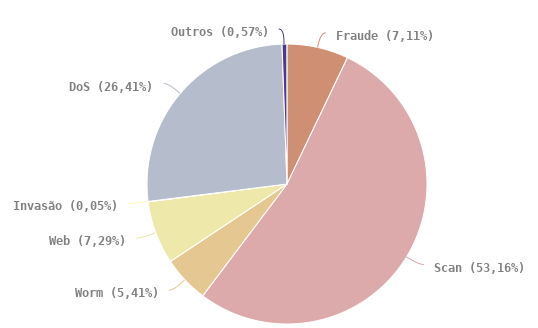
\includegraphics[scale=.6]{incidentes-reportados.png}
 \legend{Fonte: \cite{tipos-ataques:certs.br}}
 \label{fig:cert}
\end{figure}

O CERT.br é o grupo de resposta a incidentes de segurança para a internet brasileira, mantido Comitê Gestor da Internet no Brasil. Atua na notificação e tratamento de incidentes de segurança dando apoio no processo de resposta. Além disso, faz um trabalho de conscientização e treinamento sobre problemas de segurança no Brasil. 

Paralelamente ao CERT.br temos o Centro de Atendimento a Incidentes de Segurança (CAIS), mantido pela Rede Nacional de Ensino e Pesquisa (RNP). O CAIS é responsável por zela pela segurança da rede Ipê (infraestrutura de rede dedicada à comunidade brasileira de ensino superior), detectando, resolvendo e prevenindo incidentes de segurança. Além disso, tem o papel de orientar (através de publicações de cartilhas) e disseminar boas práticas de segurança da informação, educando e conscientizando usuários de todos os níveis sobre os principais riscos em segurança da informação \cite{cais}.

Desde 2008, todas a fraudes identificadas pelo CAIS estão sendo ordenadas e disponibilizadas para consulta (\autoref{fig:cais}). Adicionalmente, são enviados alertas através de uma lista quando uma fraude mostra-se particularmente perigosa aos usuários e computadores.

\begin{figure}[!htb]
 \centering
 \caption{Estatísticas de incidentes reportados ao CAIS}
 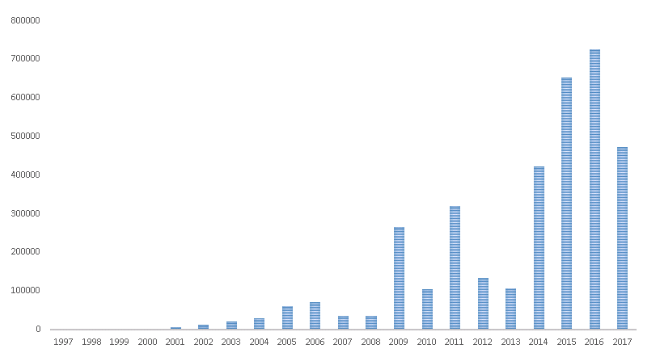
\includegraphics[scale=.7]{cais-incidentes-reportados.png}
 \legend{Fonte: \cite{cais}}
 \label{fig:cais}
\end{figure}

As empresas, de qualquer segmento e tamanho, devem ter o trabalho de manter os ativos seguros e isso vai além da utilização de anti-vírus nos computadores. Ter uma política de atualização de \textit{software} em estações de trabalho e servidores, aliados com boas práticas nas configurações de serviços, dificultam a exploração de vulnerabilidades. 

A utilização de \textit{firewall}, não pode ser encarado com uma solução definitiva, passando uma falsa sensação de segurança, pois muitas portas legítimas podem estar vulneráveis, como acontece, por exemplo, com a porta 80 que hospeda \textit{websites} vulneráveis \cite{analisenessus:cleriston}.

Diante desse cenário, torna-se cada vez mais importante para o administrador de rede e/ou segurança da informação o uso de ferramentas de IDPS, permitindo identificar e tratar de forma automatizada os incidentes de segurança.

Para implementa tais ferramentas em uma rede, deve-se levar em consideração a flexibilidade e a administração simplificada para não resultar que a empresa/instituição fique na dependência de um único fabricante ou fornecedor da solução. Além disso, a ferramenta deve ter um bom desempenho e eficiência para não passar a falsa sensação de proteção ou degradar o desempenho da rede.

\section{Motivação} \label{sec:motivação} 

A motivação desse trabalho surgiu da necessidade de implantação de um Sistema de Detecção e Prevenção de Intrusão por parte da recém formada equipe de segurança da Universidade Federal do Pará (UFPA). Tal necessidade visa melhorar a segurança de modo geral da rede acadêmica da instituição. 

Assim, diante de uma pesquisa e devido questões orçamentárias, procurou-se ferramentas de uso gratuito e com bom desempenho, capaz de atender, de forma satisfatória, as necessidades da instituição. 

Como desdobramento, encontrou-se duas ferramentas, o Snort, que se encontra no mercado desde 1998, foi a primeira no seu segmento a realizar análise de tráfego em tempo real, e o Suricata, lançado em 2010, com uma arquitetura similar ao Snort, no entanto, utiliza \textit{multithreading}, visando melhorar ainda mais o desempenho.

\section{Objetivos} \label{sec:objetivos}

Este trabalho tem como objetivo geral, avaliar e fazer um comparativo entre as soluções de código aberto de Sistemas de Detecção e Prevenção de Intrusão: Snort e Suricata. Como desdobramento de tal objetivo, os seguintes objetivos secundários foram definidos:

\begin{alineas}
\item Apresentar conceitos sobre segurança da informação e sua importância em um ambiente corporativo;
\item Descrever problemas relacionados a ataques envolvendo redes de computadores;
\item Descrever as ferramentas, compreendendo requisitos, características, modos de atuação e funcionalidades;
\item Descrever o ambiente experimental;
\item Realizar experimentos e coletar dados para validar o funcionamento e a eficiência das ferramentas;
\end{alineas}

\section{Metodologia} \label{sec:metodologia}

O método de pesquisa utilizado é o qualitativo, apoiando-se em técnica de coleta e análise de dados a partir de ferramentas. O estudo foi desenvolvido a partir de:

\begin{alineas}
\item Pesquisa bibliográfica: Os conceitos e referencias teóricos para entendimento do trabalho analisados foram: "Redes de Computadores", documentação e trabalhos referentes as ferramentas em estudos e a cartilha do CERT.br que descreve os ataques lançados as redes;
\item e a pesquisa de campo feita através da implementação de uma infraestrutura capaz de coletar dados, utilizando ferramentas auxiliares, sobre os objetos estudados.
\end{alineas}

A infraestrutura montada utiliza várias tecnologias, dentre elas temos virtualização, monitoramento de servidores, espelhamento de tráfegos de rede, etc. Para obter uma conclusão, os dados coletados foram comparados e ao final verificou-se quais das ferramentas obtiveram melhores resultados.

\section{Trabalhos Relacionados} \label{sec:trabalhos-relacionados}

O uso de ferramentas IDS \textit{opensource} Snort e/ou Suricata, importantes na área de segurança, já foi abordado e apresentou alguns resultados satisfatórios em pesquisas anteriores, por exemplo, nas pesquisas de Nagahama \textit{et al.} (2013) e Cléber \textit{et al} (2014).

%Martín \textit{et al.} (2014) e 

No trabalho do Nagahama \textit{et al.} (2013), é usado redes definidas por \textit{softwares}, que desacopla os planos de controle e de dados, permitindo adaptar o funcionamento da rede de acordo com a necessidade de cada um. O \textit{software} utilizado na pesquisa foi o OpenFLOW. Tal uso, tem como objetivo mitigar a falta de integração do IDS com os equipamentos de rede como {switches} e roteadores, o que limita a atuação destas ferramentas. 

O trabalho do Nagahama foi de fundamental importância para o entendimento dos conceitos relacionados a Sistemas de Detecção e Prevenção de Intrusão, dando uma explanada breve sobre as ferramentas Snort e Suricata. No entanto, ele não faz um comparativo de desempenho entre as ferramentas proposto nesse trabalho.

%Já Martín \textit{et al.} (2014), utiliza-se do BroFlow que possui uma série de vantagem, como, detecção de intrusão através de algoritmos simples, modular e flexível, reação imediata a um ataque descantando pacotes dos atacantes os mais próximo da origem. Dentre os resultados obtidos, destacam-se que a ferramenta conseguiu garantir o encaminhamento de pacotes legítimos na rede na taxa máxima do enlace e reduziu, em até dez vezes, o atraso na rede provocado pelo ataque.

Já Cléber \textit{et al} (2014), foi feito uma comparação de desempenho das ferramentas de IDS (Snort e Suricata) porém usou-se dados sintéticos fornecidos pela \textit{Defense Advanced Research Projects Agency} (DARPA) e devido ser uma base com ataques antigos, não houve resultados satisfatórios. Ao final, listou-se as vantagens e desvantagens existentes de cada ferramenta. No trabalho proposto, no entanto, serão usados dados mais próximo de um ambiente de produção de um rede acadêmica. 

\section{Organização do Trabalho} \label{sec:organização-do-trabalho}

O restante desse trabalho está organizado da seguinte forma.

No \autoref{ch:segurança}, são definidos conceitos sobre redes de computadores e segurança da informação, também são descritos os ataques comuns e ferramentas utilizadas para validar e avaliar as soluções de IDPS.

Em seguida, no \autoref{ch:idps}, a definição IDPS, os tipos existentes, as funcionalidades e descrição das ferramentas avaliadas: Snort e Suricata.

O \autoref{ch:cenário-real} detalhará o cenário real e a infraestrutura utilizada para os realização dos testes das ferramentas, os testes realizados e o resultados obtidos.

Por fim, no \autoref{ch:considerações}, as considerações finais e trabalhos futuros.

\chapter{Segurança em Redes de Computadores} \label{ch:segurança}

Este capítulo esta organizado da seguinte forma: A próxima seção apresenta as definições sobre segurança da informação. Na \autoref{sec:cenario-geral} será apresentado uma topologia de rede comum, que existe na organizações. Na \autoref{sec:pontos-vulnerabilidade} será abordado os pontos vulneráveis em um rede. Na \autoref{sec:ataques-comuns} será apresentado o principais ataques a rede de computadores. Por fim, na \autoref{sec:ferramentas} será apresentada as ferramentas usadas para gerar os ataques.

\section{Definições} \label{sec:definições}

Nessa seção será apresentada os principais sobre segurança da informação. Para tal, precisamos conceituar alguns termos apresentados abaixo \cite{esr-gestao}:

\begin{alineas}
\item \textbf{Incidente de segurança}: qualquer evento oposto a segurança; por exemplo, ataques de negação de serviços (\textit{Denial of Service} - DoS), roubo de informações, vazamento e obtenção de acesso não autorizado a informações;
 \item \textbf{Ativo}: qualquer coisa que tenha valor para a organização e para seus negócios. Alguns exemplo: banco de dados, softwares, equipamentos (computadores e notebooks), servidores, elementos de redes (roteadores, switches, entre outros), pessoas, processos e serviços;
 \item \textbf{Ameaça}: qualquer evento que explore vulnerabilidades. Causa potencial de um incidente indesejado, que pode resultar em dano para um sistema ou organização;
 \item \textbf{Vulnerabilidade}: qualquer fraqueza que possa ser explorada e comprometer a segurança de sistemas ou informações. Fragilidade de um ativo ou grupo de ativos que pode ser explorada por uma ou mais ameaças. Vulnerabilidades são falhas que permitem o surgimento de deficiências na segurança geral do computador ou da rede. Configurações incorretas no computador ou na segurança também permitem a criação de vulnerabilidades. A partir dessa falha, as ameaças exploram as vulnerabilidades, que, quando concretizadas, resultam em danos para o computador, para a organização ou para os dados pessoais;
 \item \textbf{Risco}: probabilidade de uma ameaça se concretizar;
 \item \textbf{Ataque}: qualquer ação que comprometa a segurança de uma organização;
 \item \textbf{Impacto}: consequência de um evento.
\end{alineas}

Segurança da Informação é a proteção das informações, sistemas, recursos e demais ativos contra desastres, erros (intencionais ou não) e manipulação não autorizada, objetivando a redução da probabilidade e do impacto de incidentes de segurança.

Segundo a norma ISO/IEC 27002 \cite{isoiec27002}, segurança da informação é a preservação da confidencialidade, da integridade e da disponibilidade da informação, adicionalmente, outras propriedades, tais como autenticidade, responsabilidade, não repúdio e confiabilidade, podem também estar envolvidas.

Dentre vários conhecimentos que um profissional de segurança deve possuir, o conceito mais básico e considerado o pilar de toda a área de segurança corresponde à sigla CID (Confidencialidade, Integridade e Disponibilidade), de modo que um incidente de segurança é caracterizado quando uma dessas áreas é afetada \cite{seg-redes-sistemas}. Abaixo será detalhado cada item.

\begin{alineas}
 \item \textbf{Confidencialidade}: termo ligado à privacidade de um ativo ou recurso, que deve ser acessível somente por pessoas ou grupos autorizados;
 \item \textbf{Integridade}: possui duas definições, a primeira está relacionada com o fato da informação ter valor correto, a segunda, está ligada à inviolabilidade da informação;
 \item \textbf{Disponibilidade}: está relacionada ao acesso à informação, que deve está disponível quando necessária.
\end{alineas}

Dois dos termos citados são fáceis de ser monitorados pois é perceptível para o usuário: a integridade (identificar se uma informação foi alterada) e a disponibilidade (tentando acessar um serviço e verificando se o mesmo está respondendo adequadamente). No entanto, só é possível identificar se houve quebra da confiabilidade através de auditorias, analisando os registros de acesso (se houver), tornando a identificação complicada e em muitos casos impossível \cite{seg-redes-sistemas}.

Além dos conceito listados, a literatura moderna considera mais alguns conceitos auxiliares, temos:

\begin{alineas}
 \item \textbf{Autenticidade}: garantia que uma informação, produto ou documento foi elaborado ou distribuído pelo autor a quem se atribui;
 \item \textbf{Legalidade}: garantia de que ações sejam realizadas em conformidade com os preceitos legais vigentes e que seus produtos tenham validade jurídica;
 \item \textbf{Não repúdio}: conceito bastante utilizado em certificação digital, onde o emissor de uma mensagem não pode negar que a enviou;
 \item \textbf{Privacidade}: habilidade de uma pessoa controlar a exposição e a disponibilidade de informações acerca de si.
\end{alineas}

Pode-se classificar os ataques em passivos e ativos. Em um ataque passivo não há interação direta (modificações de arquivos ou afetando os recursos) com o sistema alvo, o atacante apenas monitora com o objetivo de obter informações. Por outro lado, os ataques ativos há modificações de dados que afetam as operações do sistema. Os ataques podem ser divididos em categorias apresentadas na tabela.

\begin{table}[htb]
\ABNTEXfontereduzida
\centering
\caption{Classificação dos ataques passivos e ativos}
\label{tab:tipos-de-ataques}
\begin{tabular}{|l|l|p{7cm}|}
    \hline
    \textbf{Ataque} & \textbf{Categoria} & \textbf{Descrição} \\
    \hline
    Passivo & Liberação de conteúdo da mensagem & Ocorre quando uma informação é captada e seu conteúdo é lido pelo atacante \\ 
    \hline
            & Análise de tráfego & Ocorre quando o tráfego da troca de uma informação (criptografada ou não) é analisado para identificar padrões nas mensagens \\
    \hline
    Ativo & Disfarce & Ocorre quando uma entidade finge ser outra entidade \\
    \hline
          & Repetição & Ocorre quando os dados são capturados passivamente e, subsequentemente, retransmitidos para produzir um efeito não autorizado \\
    \hline
          & Modificação da mensagem & Ocorre quando alguma parte da mensagem original é alterada para produzir um efeito não autorizado \\
    \hline
          & Negação de serviço & Ocorre quando há um impedimento ou inibição do uso ou gerenciamento normal das instalações de comunicação \\
    \hline
\end{tabular}
\legend{Fonte: Autoria própria} 
\end{table}

\section{Cenário Geral} \label{sec:cenario-geral}

Nessa seção será explicado alguns conceito básico sobre redes de computadores e descrever uma topologia de rede genérica conectada a internet.

Uma rede de computadores é um conjunto de dispositivos interconectados para compartilhar recursos como \textit{hardware}, \textit{software}, interação e interatividade, onde existem máquinas que desempenham os papéis de clientes, servidores e/ou parceiros dependendo do serviços disponíveis na rede \cite{modelo:jose}.

As características de uma rede são: dois ou mais computadores interligados; meio físico de comunicação (com fio, sem fio, metálico, fibra, etc); vários tipos de equipamentos (estações de usuários, servidores, concentradores, etc); software para comunicação entre os equipamentos (protocolos); aplicativos para transferência de informação \cite{esr:arquitetura}.

As redes podem ser classificadas em duas categorias \cite{esr:arquitetura}: 
\begin{alineas}
\item \textbf{Redes par-a-par ou peer-to-peer}: Aqui não existem servidores dedicados ou hierarquia entre os computadores, todos são iguais, onde cada computador funciona como cliente e/ou servidor, cabendo o usuário determinar o que será compartilhado;
\item \textbf{Redes cliente-servidor}: Aqui há servidores dedicados que oferecem serviços à rede (servidores de arquivos e impressão, correio, fax, comunicação, aplicações, etc), geralmente são otimizadas para processar rapidamente as requisições dos clientes da rede e para garantir a segurança dos arquivos e pastas.
\end{alineas}

\begin{figure}[htb]
 \label{fig:arq-redes}
 \centering
 \begin{minipage}{0.4\textwidth}
  \centering
  \label{fig:p2p}
  \caption{Rede par-a-par}
  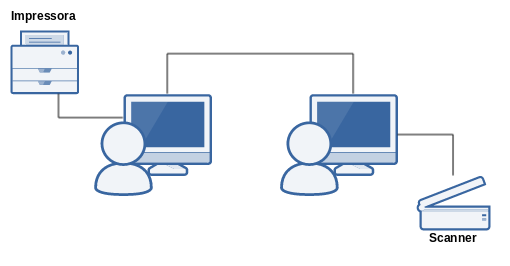
\includegraphics[scale=.4]{p2p.png}
  \legend{Fonte: Autoria própria}
 \end{minipage}
 \hfill
 \begin{minipage}{0.4\textwidth}
  \centering
  \label{fig:cliente-servidor}
  \caption{Rede cliente-servidor}
  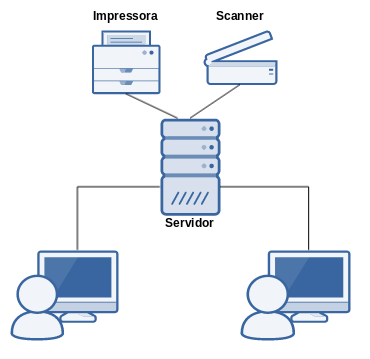
\includegraphics[scale=.4]{cliente-servidor.png}
  \legend{Fonte: Autoria própria}
 \end{minipage}
\end{figure}

Uma Internet é uma rede de computadores que interconecta centenas de dispositivos de computadores ao redor do mundo \cite{redes:kurose}. A União Internacional de Telecomunicações (UTI) estima que haja cerca de 3.578 milhões (\autoref{fig:estatisca-itu}) de usuários usando diferentes tipos de dispositivos, como, celulares, automóveis, \textit{webcams}, TVs, \textit{laptops}, consoles para jogos, entre outros \cite{estatistica:itu}.

\begin{figure}[htb]
    \centering
    \caption{Quantidade de usuário conectados na Internet} 
    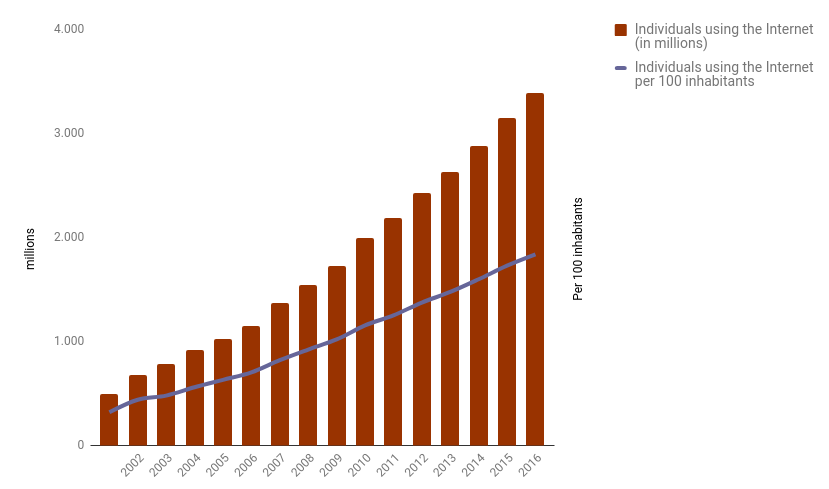
\includegraphics[scale=.55]{estatistica-uit.png}
    \legend{Fonte: \cite{estatistica:itu}}
    \label{fig:estatisca-itu}
\end{figure}

Os equipamentos que são comumente usados nas redes de computadores são:

\begin{alineas}
\item \textbf{Concentradores (\textit{hubs})}: São pontos de conexões para dispositivos em uma rede, contendo várias portas usados para conectar os segmentos da LAN. Quando um pacote chega em uma porta, ele é replicado para as demais portas, assim, todos os clientes conectados ao \textit{hub} podem ver todos os pacotes. Esse tipo de equipamento não é mais recomendado.
\item \textbf{Switches}: São equipamentos que se diferem dos \textit{hubs} por serem capazes de ler o MAC de origem e destino. Além disso, realizam comutações (os pacotes são individualmente encaminhadas entre os dispositivos conectados) de quadros na camada de enlace;
\item \textbf{Roteadores}: São dispositivos de rede mais tradicionais, como de backbone das intranets e da internet. Suas principais funções são seleção dos melhores caminhos de saída para os pacotes de entrada e roteamento destes pacotes para a interface de saída apropriada.
\end{alineas}

Um administrador, com o minimo de consciência sobre segurança, coloca em sua rede, um \textit{firewall} de borda. Um \textit{firewall} sempre é colocada na divisa entre duas ou mais redes, pode ser entre redes privadas ou entre uma rede privada e a Internet. Uma empresa pode ter muitas LANs conectadas de forma arbitrárias, mas todo o tráfego de saída ou de entrada da empresas para a internet deve ser feito através do \textit{firewall}, permitindo assim, que alguns pacotes passem e bloqueando outros \cite{redesdecomputadores}.

Há três tipos básicos de \textit{firewall}, os mais tradicionais são os filtros de pacotes e os \textit{proxies}. O terceiro tipo é uma evolução do filtro de pacotes tradicional chamado de filtro de estados de pacotes ou \textit{stateful packet filter} (SPF) \cite{univhacker}.

Um \textit{firewalls} de filtros de pacotes são baseados em tabelas configuradas pelo administrador da rede. Essas tabelas listam as origens e os destinos aceitáveis e/ou bloqueados e as regras padrões que orientam o que deve ser feito com os pacotes recebidos de outras máquinas ou destinados a elas, ou seja, o \textit{firewall} tem como função controlar o tráfego entre as redes \cite{redesdecomputadores}. 

Há vários \textit{softwares} que implementam filtro de pacotes. Alguns são instalados em \textit{hardwares} como roteadores outros são programas que rodam em computadores comuns \cite{univhacker}. Um utilitário bastante conhecido e utilizado para essa finalidade é o \textit{iptables}. A \autoref{tab:firewall-regras} apresenta um exemplo de uma tabela de regras.

\begin{table}[htb]
\ABNTEXfontereduzida
\centering
\caption{Tabela de regras aplicadas no \textit{firewall}}
\label{tab:firewall-regras}
\begin{tabular}{l|l|l|l|l|l|l}
    \textbf{IP Origem} & \textbf{IP Destino}  & \textbf{Porta Origem}  & \textbf{Porta Destino} & \textbf{Protocolo} & \textbf{Flag TCP} & \textbf{Ação} \\
    Rede Externa & Servidor Web & Todas & 80,443 & TCP & Todos & Permitir \\
    Rede Externa & Servidor Web & Todas & 21,3000:3070 & TCP & Todos & Permitir \\
    Todas & Todas & Todas & Todas & Todos & Todos & Negar \\
\end{tabular}
\legend{Fonte: Autoria própria} 
\end{table}

No exemplo, são permitidas conexões na Intranet no Servidor Web pelas portas 80 e 443 (padrão nos protocolos HTTP e HTTPS) para todos os \textit{Flags} TCP (ACK, ACK/SYN, SYN e FIN). Além disso, podemos definir um range de portas, como na linha 2, que são abertas as portas 21 e todas as portas entre 3000 e 3070, utilizadas por padrão pelo protocolo FTP.

Um \textit{proxie} trabalha na camada de aplicação interagindo com o programa e seus protocolos, independente de como esse protocolo será encapsulado na pilha TCP/IP. Por exemplo, um \textit{proxy} para Web trabalha apenas com o protocolo HTTP, bloqueando os demais. Além disso, pode-se configurar-lo para controlar quem pode ou não acessar serviços externos \cite{univhacker}.

No \textit{firewall} de filtros de pacotes por estado (SPF) uma nova tecnologia de análise de pacotes foi agregada, permitindo que eles lembrem-se de pacotes anteriores antes de permitir outro mais recente entrar. Isso é implementado na forma de uma tabela de conexões ativas. Quando uma conexão é iniciada, todos os dados do pacote são guardados nela. Se um novo pacote chegar em direção à mesma máquina, o SPF consulta a tabela. O novo pacote e aceito caso seja dada a continuação da conexão ou rejeitado, se não for \cite{univhacker}.

Na \autoref{fig:cenario-geral} apresenta uma típica rede composta por um roteador de núcleo que interliga roteadores (A, B e C) de outras redes da Intranet, que por sua vez interliga os clientes e/ou servidores. Todo trafego de saída e entrada da Intranet para a Internet passa pelo roteador de núcleo, além disso, os pacotes são tratados por um \textit{firewall} de borda, que determina o que entra e o que sai da rede local.

\begin{figure}[!htb]
    \centering
    \caption{Topologia geral de uma rede de computadores} 
    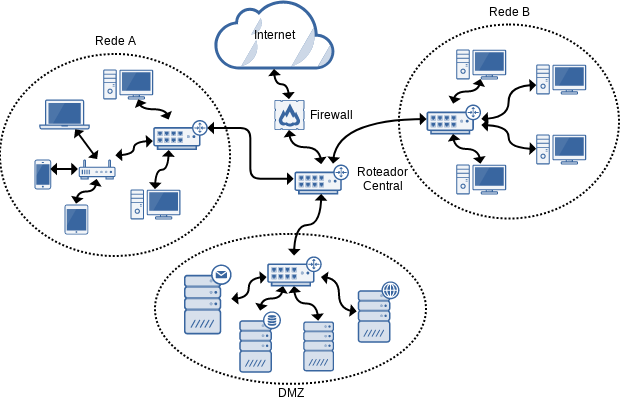
\includegraphics[scale=.6]{cenario-geral.png}
    \legend{Fonte: Autoria própria}
    \label{fig:cenario-geral}
\end{figure}

\section{Pontos de Vulnerabilidade} \label{sec:pontos-vulnerabilidade}
%Ex.: Roteador, firewall, clientes e suas aplicações, serviço mal configurado (sem aplicação de patch de atualização)
% falar dos problemas nas aplicações (erro de programação, sqlinjection, cross-site script)
% problemas relacionados a firewall que na sua maioria é fitro de pacotes, o atacante pode usar portas abertas no firewall que possuem serviços com falhas de segurança conhecidas ou aplicações mal desenvolvidas.
% clientes, envolve engenharia social, mencionar senha fraca, prática de spam

Nessa seção será abordado os pontos fracos que uma pessoa má intencionada pode explorar para ter um ataque bem sucedido a um rede de computador.

Apesar da preocupação dos administradores em proteger suas redes de ataques, devido a sua heterogeneidade, sempre haverá uma breja a ser explorada. A literatura considera o ser humano como elo mais fraco, é bastante comum o usuário cadastrar senhas fracas, por conveniência, e fácil memorização (\autoref{sec:forçabruta}).

%phishing e spam 

Outro problema comum é o desenvolvimento de aplicações \textit{web} sem nenhuma preocupação com segurança, podendo comprometer, não somente o serviço, mas também, em casos mais extremos, o servidor inteiro. Para tal, atacante pode usar vários artifícios, os mais conhecidos são \textit{sql injection} e \textit{cross-site script}.

A inserção de Structured Query Language (SQL) via formulário na aplicação \textit{web} resulta num ataque de \textit{sql injection}. O atacante injeta um código dentro dos campos de entrada, como usuário e senha, de uma aplicação onde a declaração condicional sempre será verdadeiro quando executado. Em casos bem sucedidos, o atacante pode alterar o banco de dados, acessar informações sensíveis ou ter acesso ao sistema \cite{sqlinjection:sankaran}.

No exemplo abaixo, a declaração condicional 'OR 1=1' torna toda a clausura WHERE verdadeiro pois a expressão 1=1 é uma tautologia. A consulta retorna todos os dados da tabela \textit{user\_info}. Perceba que os dois hífens fornecidos no final da entrada comenta o resto da linha.

\begin{lstlisting}[Language=SQL]
  SELECT * FROM user_info WHERE logID="" OR 1=1 -- AND pass1="" 
\end{lstlisting}

O \textit{Cross-site scripting} (XSS) é uma forma de ataque que permite utilizar um aplicação vulnerável para transporta códigos maliciosos até o navegador de outros usuário. O navegador da vítima entende que o código recebido é legítimo e, por isso, informações sensíveis, como o identificador de sessão do usuário, por exemplo, podem ser acessadas programaticamente \cite{pentestweb:nelson}.

Com o XSS pode-se roubar histórico de navegação, fazer uma varredura de redes privadas, descobrir consultas realizadas em mecanismos de busca, escravizar o navegador \textit{web} e proliferar \textit{worms} (\autoref{sec:malwares}) baseados em XSS \cite{pentestweb:nelson}. 

\section{Ataques Comuns à Redes de Computadores} \label{sec:ataques-comuns}

Nessa seção será descritos os ataques mais comuns à redes e serviços de organizações privadas e públicas, financeiras ou acadêmicas. Para licitar os ataques dessa seção, levou-se em consideração as estatísticas divulgada pelo CERT.br (\autoref{fig:cert}).

O CERT.br é o grupo de resposta a incidentes de segurança para a internet brasileira, mantido Comitê Gestor da Internet no Brasil. Atua na notificação e tratamento de incidentes de segurança dando apoio no processo de resposta. Além disso, faz um trabalho de conscientização e treinamento sobre problemas de segurança no Brasil. 

\begin{figure}[htb]
 \centering
 \caption{Estatísticas de ataques reportadas ao CERT.br}
 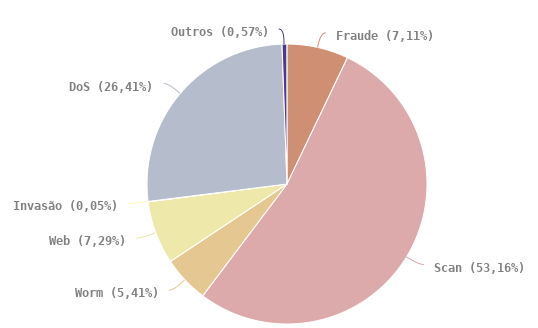
\includegraphics[scale=.6]{incidentes-reportados.png}
 \legend{Fonte: \cite{tipos-ataques:certs.br}}
 \label{fig:cert}
\end{figure}

Paralelamente ao CERT.br temos o Centro de Atendimento a Incidentes de Segurança (CAIS), mantido pela Rede Nacional de Ensino e Pesquisa (RNP). O CAIS é responsável por zela pela segurança da rede Ipê (infraestrutura de rede dedicada à comunidade brasileira de ensino superior), detectando, resolvendo e prevenindo incidentes de segurança. Além disso, tem o papel de orientar (através de publicações de cartilhas) e disseminar boas práticas de segurança da informação, educando e conscientizando usuários de todos os níveis sobre os principais riscos em segurança da informação \cite{cais}.

Desde 2008, todas a fraudes identificadas pelo CAIS estão sendo ordenadas e disponibilizadas para consulta (\autoref{fig:cais}). Adicionalmente, são enviados alertas através de uma lista quando uma fraude mostra-se particularmente perigosa aos usuários e computadores.

\begin{figure}[htb]
 \centering
 \caption{Estatísticas de incidentes reportados ao CAIS}
 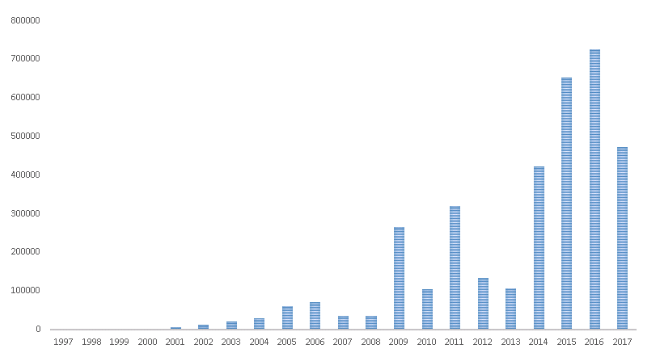
\includegraphics[scale=.7]{cais-incidentes-reportados.png}
 \legend{Fonte: \cite{cais}}
 \label{fig:cais}
\end{figure}

\subsection{\textit{Scanners}} \label{sec:scanners}

Conforme tratado na \autoref{sec:definições}, uma vulnerabilidade é a fraqueza em sistemas de informação, procedimentos de segurança do sistema e controles internos, ou aplicação que pode ser explorada tendo como origem uma ameaça. 

\textit{Scanners} são programas usados para varrer uma rede à procura de computadores (tanto pessoais como servidores) com alguma vulnerabilidade. Podemos dividir os \textit{scanners} em dois tipos \cite{univhacker}: 

\begin{alineas}
\item \textbf{\textit{scanner} de portas TCP/IP abertas (ou \textit{portscanner})}: cada serviço de rede que estiver disponível em uma determinada máquina é uma porta de entrada em potencial. Existem um total de 128 mil porta, sendo 65536 portas para o protocolo TCP e 65536 portas para o protocolo UDP. O \textit{portscanner} verifica quais portas TCP/IP estão abertas com o objetivo de determinar quais serviços de rede TCP/IP disponíveis. Quase todas as técnicas de \textit{portscanning} valem-se de sinais (ou \textit{flags}), TCP, UDP ou ICMP, e a partir da análise desses sinais, os \textit{scanners} retiram informações sobre o sistema; \cite{univhacker}
\item \textbf{\textit{scanner} de vulnerabilidades conhecidas}: Um vez determinados os serviços que uma máquina disponibiliza na rede entra em cena o \textit{scanner} de vulnerabilidade. A ideia é checar, através de uma lista de falhas conhecidas, se o sistema está ou não executando um serviço com problemas \cite{univhacker}. 
\end{alineas}

Normalmente, essas ferramentas funcionam em três estágios \cite{avaliacao:tania}:

\begin{alineas}
 \item \textbf{Configuração}: aqui será definido o endereço IP do alvo ou a URL (Uniform Resource Locator) da aplicação Web e demais parâmetros, como, por exemplo, utilização de \textit{proxy}.
 \item \textbf{Rastreamento}: esse estágio, em \textit{scanners} de vulnerabilidade de aplicações web, o \textit{scanner} chama a primeira página web e então examina seu código procurando \textit{links}. Cada \textit{link} encontrado é registrado e este procedimento é repetido várias vezes até que \textit{links} e páginas não sejam mais encontrados.
 \item \textbf{Exploração}: vários testes são executados e as requisições e respostas são armazenadas e analisadas. Ao final, os resultados são exibidos ao usuário e podem ser salvos para uma análise posterior. 
\end{alineas}

Um bom \textit{scanner} de vulnerabilidade verifica itens como \cite{univhacker}: 

\begin{alineas}
\item \textbf{Erros comuns de configuração}: portas não utilizadas por nenhum serviço abertas;
\item \textbf{Configurações e senhas-padrões}: instalação de softwares deixando-os com as configurações de fabrica (com usuário e senha-padrão), por exemplo, usuário: admin, senha: admin. Outro problema é deixar serviços desnecessários ativados;
\item \textbf{Combinação óbvias de usuário e senha}: Usuário comuns tendem a colocar senhas fáceis de lembrar;
\item \textbf{Vulnerabilidades divulgadas}: Sempre que uma falha de segurança é divulgada há uma corrida dos desenvolvedores para saná-las. Em paralelo, existem \textit{hackers} que querem chegar aos sistemas vulneráveis antes de serem consertados.
\end{alineas}

Os \textit{scanners} de vulnerabilidades automatizados contêm, e atualizam regularmente, enormes bancos de dados de assinaturas de vulnerabilidades conhecidas para basicamente tudo o que está recebendo de informações em uma porta de rede, inclusive sistemas operacionais, serviços e aplicativos web \cite{hackers:stuart-joel}. 

\subsection{\textit{Exploit}} \label{sec:exploit}

Os atacantes exploram \textit{bugs} ou vulnerabilidades em programas para ter acesso ao sistema alvo. Infelizmente, existem milhares de \textit{bugs}, em 2013, por exemplo, foram reportados 103,000 \textit{bugs} no sistema operacional Ubuntu. Outro projetos de códigos fechados, possuem estatísticas similares \cite{aeg:thanassis}.

Diante das vulnerabilidades obtidas por um \textit{scanners} (\autoref{sec:scanners}), o passo seguinte seria usar um \textit{exploit} adequado. Os \textit{exploit} são pequenos utilitários usados para explorar vulnerabilidades específicas, podendo ser utilizados de forma \textit{"stand alone"}, ou seja, diretamente, ou podem ser incorporados à \textit{malwares} \cite{exploit:cassio}.

Para alguns \textit{exploits} funcionar, é necessário ter acesso ao \textit{shell} da máquina-alvo. Tal artificio pode ser conseguido através da execução de um cavalo de tróia (\autoref{sec:malwares}) pela vítima em seu sistema. O \textit{trojan} abre uma porta de comunicação e permite que o invasor tenha total controle sobre a máquina, dessa forma é possível executar \textit{exploits} para quebrar outros níveis de segurança \cite{univhacker}.

\subsection{Força Bruta} \label{sec:forçabruta}

Na segurança da informação, a autenticação é umas das áreas-chaves onde há a distinção de usuários autorizados de outros não-autorizados, tendo como principal vantagem ser de fácil implementação, não requerendo equipamentos, como leitores biométricos \cite{denise-lilian}.

Na literatura sobre segurança da informação, o fator humano é considerado o elo mais fraco. Muitos usuários, por conveniência, criam senhas de acesso fáceis e, em muitos casos, única para acessar diversos sistemas. Nesse ponto que \textit{hackers} iram atuar para ter acesso não-autorizado ao sistema. 

Existem três métodos mais usados por programas de quebra de senha: ataques de dicionário (ou lista de palavras), ataques híbridos e ataques de força-bruta. Nos ataques por dicionários, utilizam-se listas de palavras comuns: nomes próprios, marcas conhecidas, gírias, nomes de canções, entre outros, tais elementos conseguidos por engenharia social \cite{univhacker}. 

 Um ataque de força bruta consiste em gerar todas as permutações e combinações possíveis de senha, criptografar cada uma e comparar a senha gerada com a senha criptografada original até encontrar uma que seja igual \cite{md5crack2012}. 

 Esse tipo de ataque é facilmente detectável pois, além de gerar uma alta carga no servidor, gera uma grande quantidade de registros de logs. No entanto, caso a pessoa má intencionada, de alguma outra forma, tenha acesso ao arquivo de \textit{hash} ou a tabela de usuário de um banco de dados, com as senha criptografadas do sistema, ela pode usar o ataque de força bruta no arquivo em qualquer máquina, assim, impossibilitando a detecção do ataque.

 Muitos sistemas já possuem formas de contornar esse tipo de ataque, por exemplo, bloqueio de usuário ao errar a palavra-chave por uma certa quantidade de vezes. Outra forma, é colocar um tempo de expiração da senha, por exemplo, a senha deve ser trocada a cada trinta dias por uma diferente e nunca usada anteriormente, dessa maneira, inviabilizando a quebra de senha por força bruta. 

 \subsection{Desfiguração de páginas} \label{sec:desfiguração}

 A desfiguração de páginas, \textit{defacement} ou pichação ocorre quando o conteúdo da página \textit{web} de um site é alterado. O atacante (\textit{defacer}) consegue fazer alterações em páginas explorando vulnerabilidade nas aplicações \textit{web} que permite injeção de \textit{script} malicioso ou através de furto de senha de acesso à interface \textit{web} usadas para administração remota \cite{certs-ataques}.

 Nos serviços \textit{web}, como por exemplo, apache2 existe um usuário especial, comumente chamado de www-data ou algo semelhante. O servidor \textit{web}, na maioria das vezes, precisa apenas de permissões de leitura nos arquivos porém muitos gerentes de sistemas cujo a conscientização sobre segurança é insuficiente, designa permissões errôneas (escrita ou alteração), e caso haja um comprometimento, através, por exemplo, de injeção de código remoto PHP, do servidor, o atacante poderá alterar a maioria dos arquivos. A ocorrência amplamente disseminada de ataques de desfiguração de páginas Web é uma consequência direta dessa prática \cite{seguranca:william-lawrie}.

 Em 2010, o site Zone-h registrou mais de 1,4 milhões de páginas desfiguradas, muitas delas associadas a ataques \textit{Cross-site scripting} (XSS). Os \textit{defacements} são considerados ataques passivos pois é gerado apenas uma mensagem na tela \cite{angelo-xss}.

 \subsection{Negação de Serviços} \label{sec:negação}
 
 Um ataque de negação de serviço (\textit{Denial of Service} - DoS) tem como principal objetivo deixar um serviço (servidor \textit{web}, banco de dados) ou recurso (memória, processador)  indisponível, impossibilitando que usuário legítimos tenham acesso a esses recursos. Para tal, o atacante gera diversas requisições inúteis para o servidor, consumindo seus recursos até que o serviço não esteja mais disponível ou degradando a qualidade do serviço \cite{cryptsec}.

 Pode-se dividir os ataques de Dos em três categorias \cite{redes:kurose}:

\begin{alineas}
\item \textbf{Ataque de vulnerabilidade}: Envolve o envio de um série de mensagens a uma aplicação ou sistema operacional vulnerável, como consequência o serviço pode parar ou, no pior caso, o hospedeiro pode pifar;
\item \textbf{Inundação na largura de banda}: O atacante envia um grande quantidade de pacotes ao hospedeiro, fazendo com que o enlace de acesso do alvo fique indisponível, impedindo os pacotes legítimos de alcançarem o servidor;
\item \textbf{Inundação na conexão}: O atacante estabelece um grande número de conexões no hospedeiro-alvo fazendo-o deixar de aceitar conexões legítimas.
\end{alineas}

Esse tipo de ataque pode gerar grandes prejuízos financeiros para as empresas, principalmente \textit{e-commence}, pois enquanto o sistema está fora ou com uma resposta lenta, as transações financeiras são prejudicadas. Com isso, cria-se também, uma insatisfação pelo usuário do serviço prestado pela empresa.

Existe uma forma mais sofisticada de ataque de DoS chamada Negação de Serviço Distribuído (\textit{Distributed Denial of Services} - DDoS), enquanto o DoS básico as requisições partem de apenas uma fonte, no entanto, no DDoS o atacante tem acesso a um grande número de computadores (\textit{zombies}) explorando suas vulnerabilidades criando o que chamamos de \textit{botnet} (\autoref{fig:ddos}). Com isso, basta o atacante indicar as coordenadas de um ou mais alvos para o ataque \cite{zargarjoshitipper}. O DDoS são mais difíceis de detectar e de prevenir do que um ataque DoS de um único hospedeiro.

\begin{figure}[htb]
 \centering
 \caption{Ataque de Negação de Serviço Distribuído}
 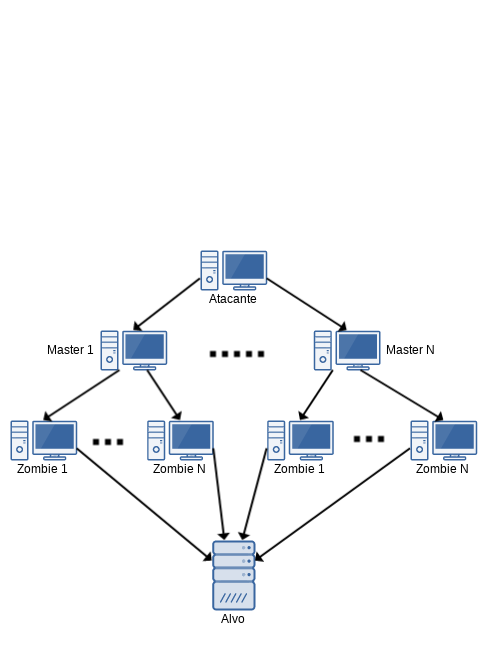
\includegraphics[scale=.6]{ddos.png}
 \legend{Fonte: Autoria própria}}
 \label{fig:ddos}
\end{figure}

\subsection{\textit{Malwares}} \label{sec:malwares}

Os \textit{malwares}, também conhecidos como \textit{softwares} maliciosos, são um grande problema para sistemas de informação, sua existência ou execução tem consequências negativas ou involuntárias. Nessa seção será apresentado os \textit{malwares} mais popularmente conhecidos que são os vírus, \textit{worms}, \textit{trojans} e, devido sua repercussão, os \textit{ransomwares}.

 É importante entender o funcionamento e o comportamento desses códigos maliciosos para, a partir daí, buscar soluções contra esse ataque. Existe dois tipos de análise: análise estática, requer uma verifica linha a linha do código malicioso, geralmente o código não está disponível e até mesmo se estiver, o autor do \textit{malware} muitas vezes ofusca o código, tornando esse tipo de análise difícil. Por outro lado, existe a análise dinâmica, o analista monitora a execução e o comportamento do \textit{malware}, esse tipo de análise é imune a ofuscação de código \cite{encycrypt}.

 O Vírus é um programa que se propaga inserindo cópias de si mesmo e se tornando parte de outros programas e arquivos. Para dar continuidade ao processo de infecção, o vírus depende da execução do programa ou arquivo hospedeiro. O principal meio de propagação desse tipo de \textit{software} malicioso são as mídias removíveis, como, por exemplo, \textit{pen-drives} \cite{certs-malwares}.

 O \textit{Worm} é um \textit{malware} que se propaga através de e-mails, sites ou \textit{software} baseados em rede, explorando as vulnerabilidades das aplicações. Uma das principais características desse tipo de \textit{software} é a propagação automática, ou seja, sem a intervenção do usuário \cite{detectingworm}. 

 O \textit{Trojan} ou Cavalo de Troia são programas que precisam ser explicitamente executados para serem instalados no computador. Esse \textit{malware} se disfarça de um programa benigno, por exemplo, cartões virtuais animados, álbuns de fotos, jogos e protetores de tela que ao serem executados o \textit{trojan} é instalado sem o consentimento do usuário. No entanto, o atacante, após invadir um computador, pode instalar o \textit{trojan} alterando as funções já existentes de programas para executarem ações maliciosas \cite{certs-malwares}.

 Por fim, temos os \textit{ransomwares}. O \textit{ransomware} é um \textit{malware} que criptografa os dados de um computador ou uma rede. A pessoa ou a organização responsável pelo ataque pede um resgate, geralmente pago em bitcoin para manter sua anonimidade, fornecendo uma chave para descriptografar os arquivos mediante o pagamento \cite{ransomware:matt}.

 A melhor medida contra esse tipo de \textit{malware}, uma vez que, não há garantias que o atacante irá fornecer a chave depois do pagamento, além de manter o sistema sempre atualizado, é ter uma politica de \textit{backup} regular. O armazenamento de arquivos importantes em outros tipos de mídias não conectadas regularmente ao sistema (removíveis) ou \textit{backup} baseados em nuvens \cite{ransomware:matt}.

 \section{Ferramentas para Avaliação de Segurança} \label{sec:ferramentas}

 Nessa seção será descrito as ferramentas auxiliares utilizadas para geração de ataques abordados na \autoref{sec:ataques-comuns} com objetivo de testar e validar as configurações das ferramentas de IDPS estudas. 

 \subsection{Nmap} \label{sec:nmap}

 O Nmap é uma ferramente de código aberto utilizada para auditoria de segurança e descoberta de rede. A ferramenta é capaz de determinar quais \textit{hosts} estão disponíveis na rede, quais serviços cada \textit{host} está oferecendo, incluindo nome e versão da aplicação, o sistema operacional usado, dentre outras características.  

 Muitos administradores de sistemas utilizam o Nmap para tarefas rotineiras como, criação de inventário de rede, gerenciamento de serviços, visto que é de suma importância manter os mesmos atualizados e monitoramento de \textit{host}.

 Diversos parâmetros podem ser utilizados com o Nmap, possibilitando realizar varreduras das mais variadas maneiras, dependendo do tipo desejado. A lista completa de opções podem ser consultadas na documentação oficial que vem junto da ferramenta ou no site do projeto \cite{nmap}. 

 Na execução do Nmap, o que não for opção ou argumento da opção é considerado especificação do \textit{host} alvo. O alvo pode ser um ou vários, usando uma notação de intervalo por hífen ou uma lista separada por vírgula. Os \textit{hosts} alvos também podem ser definidos em arquivos.

 O resultado do Nmap é uma tabela de portas e seus estados (\autoref{fig:nmap-exemplo}). As portas podem assumir quatro estados, temos: aberto (\textif{open}), significa que existe alguma aplicação escutando conexões; filtrado (\textit{filtered}), há um obstáculo na rede, podendo ser algum \textit{firewall}, que impossibilita que o Nmap determine se a porta está aberta ou fechada; fechado (\textit{closed}), não possui aplicação escutando na porta; não-filtrado (\textit{unfilterd}), a porta responde requisição porém o Nmap não consegue determinar se estão fechadas ou abertas \cite{nmap}

 \begin{figure}[htb]
  \centering
  \caption{Exemplo de saída do Nmap}
  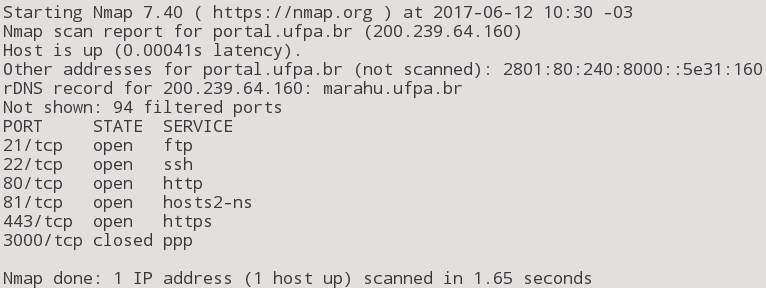
\includegraphics[scale=.5]{nmap.png}
  \legend{}
  \label{fig:nmap-exemplo}
 \end{figure}

 \subsection{Metasploit Framework} \label{sec:metasploit}

 O Metasploit é um \textit{framework} de código aberto cujo principio básico é desenvolver e executar \textit{exploit} contra alvos remotos e fornecer uma lista de vulnerabilidades existentes no alvo. É uma ferramenta que combina diversos \textit{exploits} e payloads dentro de um local, ideal para levantamento de segurança de serviços e testes de penetração \cite{metasploit:yash}.  

 O Metasploit possui uma biblioteca divida em três partes: \textbf{Rex}: É a biblioteca fundamental, a maioria das tarefas executadas pelo \textit{framework} usaram essa biblioteca; \textbf{MSF Core}: É o \textit{framework} em si, possui, por exemplo, gerenciador de módulos e a base de dados; \textbf{MSF Base}: Guarda os módulos, sejam eles, \textit{exploit}, \textit{encoders} (ferramentas usadas para desenvolver o \textit{payloads}) e os \textit{payloads}. Além disso, são guardadas informações de configuração e sessões criadas pelos \textit{exploits}. A arquitetura é mostrada com mais detalhes na \autoref{fig:metasploit-arquitetura}. 

 Os módulos são divididos da seguinte maneira: Payload: são código executados no alvo remotamente; Exploit: explora \textit{bugs} ou vulnerabilidade existente em aplicações do alvo; Módulos Auxiliares: usado para escanear as vulnerabilidades e executar várias tarefas; Encoder: codifica o \textit{payload} para evitar qualquer tipo de detecção pelo anti vírus.

 \begin{figure}[!htb]
  \centering
  \caption{Arquitetura do Metasploit}
  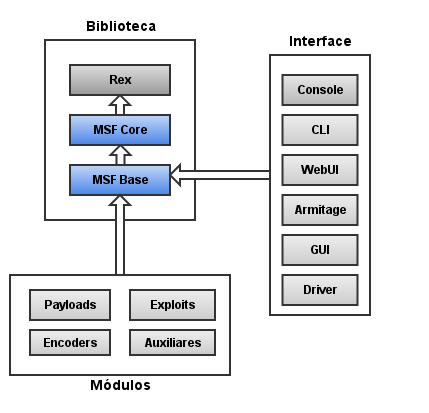
\includegraphics[scale=.6]{metasploit_arquitetura.png}
  \legend{Fonte: Autoria própria}
  \label{fig:metasploit-arquitetura}
 \end{figure}

 \subsection{Pytbull} \label{sec:pytbull}

 O Pytbull é um \textit{framework} para teste de IDPS, capaz de determinar a capacidade de detecção e bloqueio do mesmo, além de fazer uma comparação entre diversas soluções e verifica as configurações \cite{pytbull}. O \textit{framework} Pytbull possui cerca de 300 testes agrupados em 11 módulos, temos:

 \begin{alineas}
  \item \textbf{badTraffic}: pacotes não compatíveis com a RFC são enviados para o servidor para testar como os pacotes são processados; 
  \item \textbf{bruteForce}: testa a capacidade do IDPS de rastrear ataques de força bruta;
  \item \textbf{clientSideAttacks}: usa um \textit{shell} reverso para fornecer ao servidor instruções para baixar arquivos maliciosos; 
  \item \textbf{denialOfService}: testa a capacidade do IDPS de proteger contra tentativas de DoS; 
  \item \textbf{evasionTechniques}: testa a capacidade do IDPS de detectar técnicas de evasão; 
  \item \textbf{fragmentedPackets}: várias cargas úteis fragmentadas são enviadas ao servidor para testar sua capacidade de recomposição e detectar os ataques; 
  \item \textbf{ipReputation}: testa a capacidade do servidor detectar tráfego de servidores com reputação baixa;
  \item \textbf{normalUsage}: cargas úteis que correspondem a uso normal; 
  \item \textbf{pcapReplay}: permite reproduzir arquivos pcap; 
  \item \textbf{shellCodes}: envia \textit{shellcodes} para o servidor na porta 21/ftp testando a capacidade de detectar e/ou bloquear o mesmo; 
  \item \textbf{testRules}, testa a base de assinaturas configuradas no servidor IDPS.
 \end{alineas}

Existem basicamente 5 tipos de testes: socket, abre um \textit{socket} em uma porta e envia o \textit{payload} para o alvo remoto na porta especificada; command, envia um comando para alvo remoto com a função python subprocess.call(); scapy, envia cargas úteis especificas baseadas na sintaxe de Scapy; client side attacks, usa um \textit{shell} reverso no alvo remoto e envia comandos para serem processados no servidor; pcap replay, permite reproduzir tráfego com base em arquivos de pcap.

 \begin{figure}[htb]
  \centering
  \caption{Arquitetura do \textit{framework} Pytbull}
  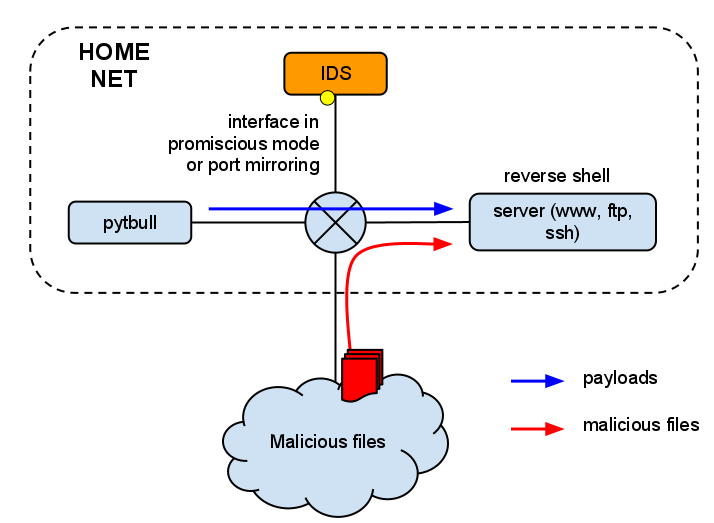
\includegraphics[scale=.4]{arquitetura_pytbull.png}
  \legend{Fonte: \cite{pytbull}}
  \label{fig:pytbull}
 \end{figure}

 \section{Conclusão}

 Este capítulo apresentou

\chapter{Sistemas de Detecção e Prevenção de Intrusão} \label{cap:idps}
 %breve texto introduzindo o capítulo + apresentação das seções

Os sistemas de detecção e prevenção de intrusão (\textit{Intrusion Detection and Prevention System} - IDS/IPS) são ferramentas de importância reconhecida pela comunidade da segurança da informação. Nesse capítulo, vamos apresentar os principais conceitos relacionados a IDS e IPS, uma breve descrição do funcionamento e classificação, para melhor entendimento das ferramentas que iremos apresentar e avaliar em um ambiente de real.

\section{Definições de IDS/IPS} \label{sec:ipds-definicoes}

 \textit{Intrusion Detection Systems} (IDS) ou Sistemas de Detecção de Intrusão (SDI) são ferramentas utilizadas para monitoramento de eventos que ocorrem em redes e sistemas computacionais, analisando sinais de possíveis ataques que podem levar a uma violação das politicas de segurança da organização, alertando os administradores do sistema que estes eventos estão ocorrendo. O \textit{Intrusion Detection Systems} (IPS) ou Sistema de Prevenção de Intrusão (SPI) possui todas as funcionalidades do IDS com uma diferença, ele é capaz de deter alguns possíveis incidentes, minimizando os impactos causados por sistemas comprometidos \cite{mukhopadhyay01}.

 Basicamente os sistemas de detecção de intrusão são compostos por quatro componentes, temos: Sensor ou Agente, responsável pelo monitoramento e analise do trafego capturado; Banco de Dados, usado como repositório das informações de eventos detectados pelos sensor ou agente que serão processados; Gestor, é o dispositivo central que recebe, analisa e gerencia as informações de eventos vindos do sensor ou agente; Console, fornece uma interface para administração e monitoramento das atividades do IDS.

 \section{Tipos de IDS/IPS} \label{sec:idps-tipos}

 Os IDSs são classificados de acordo com o local onde o sensor é instalado, \textit{Host Based Intrusion Detection Systems} (HIDS) e \textit{Network Based Intrusion Detection Systems} (NIDS), e a técnica utilizada para o monitoramento, baseado em assinaturas e anomalias \cite{nagahama2012ipsflow}.

 Em um HIDS o sensor é instalado no \textit{host} que será monitorado, analisando as informações contidas na própria máquina. Esse tipo de IDS tem o objetivo de analisar aspectos internos ao \textit{host} como processos em execução, modificações na configuração do sistema e serviços, monitorar o tráfego de rede somente do \textit{host} e acesso a arquivos não autorizados, entre outros.

 Os HIDS possuem algumas vantagens como evitar que alguns códigos sejam executados; bloqueia o tráfego de entrada e saída contendo ataques e uso não autorizado de protocolos e programas; evita que arquivos possam ser acessados, modificados e deletados impedindo o instalação de \textit{malware} e outros ataques envolvendo acesso inapropriado a arquivos. Por outro lado, um HIDS possui algumas limitações como, por exemplo, difícil instalação e manutenção; interferir no desempenho do \textit{host}; demora para identificar alguns eventos consequentemente a resposta a esses incidentes sofrerá um \textit{delay} \cite{scarfone01}.

 Já em um NIDS, o sensor é instalado na rede e a interface de rede atua em um modo especial chamado ``promíscuo'', passando a ter a capacidade de capturar o tráfego da rede mesmo que os pacotes não sejam destinados ao próprio sensor.

Quanto a localização o NIDS pode ser classificado como passivo ou ativo. No modo passivo, o IDS monitora copias dos pacotes da rede que passam pelo \textit{switch} ou \textit{hub} onde está conectado, ficando limitado somente a gerar notificações quando encontrado algum tráfego malicioso. Enquanto no modo ativo, o IDS é instalado da forma que o tráfego da rede passe através do sensor parecendo com o fluxo de dados associado com um \textit{firewall}. Dessa forma, ele é capaz de parar ataques bloqueando o fluxo malicioso. 

 Os NIDS possuem algumas vantagens como serem independentes de plataforma; não interfere no desempenho do \textit{host}; fácil implantação e transparente para o atacante. Por outro lado, possuem desvantagens como: pode adicionar retardados nos pacotes quando instalado no modo ativo, isso ocorre principalmente se houver um subdimensionamento do \textit{hardware}; dificuldade de tratar dados de redes de alta velocidade; quando em modo passivo, trata apenas o segmento da rede que o IDS esta instalado e dificuldade de tratar dados criptografados. Esse tipo de IDS é mais utilizado devido a grande heterogeneidade de dispositivos e sistemas operacionais disponíveis na rede, tornando a administração mais simples se comparados com o HIDS.

 Quanto a técnica de monitoramento utilizado, o IDS pode ser baseados em assinaturas ou anomalias. IDSs baseados em assinaturas compara os pacotes com uma base de assinaturas de ataques previamente conhecidos e reportados por especialistas, cada assinatura identifica um ataque. Tem como vantagem, usar poucos recursos do servidor e rápido processamento. Porém, as desvantagens são: exigi uma atualização constante da base de assinaturas; alto conhecimento para geração da base e possuir um alto índice de falsos positivos e negativos.

 Já os baseados em anomalias, procuram determinar um comportamento normal na fase de aprendizagem do sistema computacional ou rede e sempre que existir um desvio desse padrão alertas são gerados. Possui a vantagem de detectar novos ataques sem necessariamente conhecer a fundo a intrusão através dos desvio de comportamento. Porém existe a desvantagem de gerar um grande número de falsos alertas em decorrência a modificações na rede ou \textit{host} nem sempre representar um tráfego malicioso. 

\begin{figure}[htb]
 \label{fig:nids-arquitetura}
 \centering
 \begin{minipage}{0.4\textwidth}
  \centering
  \label{fig:nids-passivo}
  \caption{Exemplo de arquitetura de NIDS passivo}
  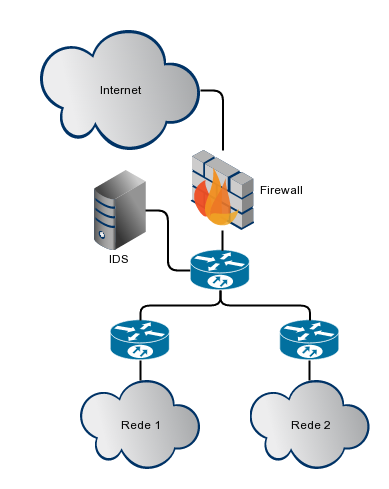
\includegraphics[scale=.55]{nids_passivo.png}
  \legend{}
 \end{minipage}
 \hfill
 \begin{minipage}{0.4\textwidth}
  \centering
  \label{fig:nids-ativo}
  \caption{Exemplos de Arquitetura de NIDS ativo}
  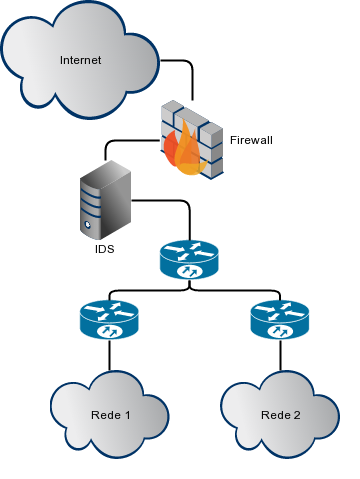
\includegraphics[scale=.55]{nids_ativo.png}
  \legend{}
 \end{minipage}
\end{figure}

\section{Principais Ferramentas de IDS} \label{sec:idps-ferramentas}
\subsection{Snort} \label{sec:snort}

O Snort é um sistema de detecção e prevenção de intrusão de código fonte aberto escrita na linguagem de programação C bem conhecido pela comunidade da segurança da informação. Seu primeiro \textit{release} foi lançado em 1998 e desde então passa por constantes revisões e aperfeiçoamentos, com o passar dos anos se tornou o IDS mais utilizado no mundo. Ele combina análise baseada em assinaturas e anomalias, podendo operar em três modos: \textit{sniffer}, \textit{packet logger} e de sistema de detecção de intrusão (NIDS) \cite{snortorgbr}.

No modo \textit{Sniffer}, o Snort captura os pacotes e exibi as informações no console. No modo \textit{Packet Logger}, além de capturar o tráfego, ele registrar essas informações em disco (arquivos de logs). E no modo NIDS, é o modo mais complexo, permite analise do pacotes de rede em tempo real.

Existe quatro componentes no Snort: O \textit{Sniffer}, o Pré-processador, o Motor de Detecção e Módulo de Saída. Os componentes são organizados de acordo com a figura \ref{snort-componentes} \cite{kohlenberg2007snort}.

 \begin{figure}[!htb]
   \centering
   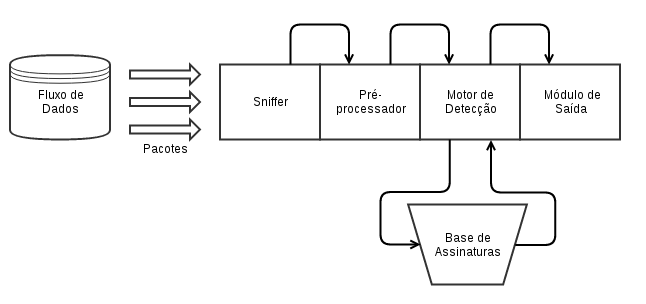
\includegraphics[scale=0.6]{snort_componentes}
   \caption{Componentes do Snort}
   \label{snort-componentes}
 \end{figure}

 \subsection{Suricata} \label{sec:suricata}
 \section{Conclusão} \label{sec:idps-conclusao}
 %Ex: Este capítulo apresentou...



\chapter{Detecção de Intrusão em um Cenário Real} \label{ch:cenário-real}
 %- Em cada capitulo adicionar um texto introdutório

Este capítulo esta organizado da seguinte forma: A próxima seção apresenta o cenário de testes, descrevendo características gerais da rede selecionada para os teste. Na seção \ref{sec:infraestrutura} será abordado a infraestrutura usada para os testes, ferramentas utilizadas e as configurações feitas. Na seção \ref{sec:testes} será descrito os testes realizados com suas respectivas justificativas. Na seção \ref{sec:resultados} será apresentado os resultados esperados e obtidos, problemas encontrados e a comparação das ferramentas e por último, na seção \ref{sec:conclusão}, uma breve conclusão.

\section{Metodologia dos Testes}

Nessa seção será descrito o cenário utilizado para a realização dos testes. Na \autoref{sec:cenário}, aborta a rede onde os sensores foram instalados e algumas de suas estatísticas de uso. A \autoref{sec:infraestrutura} descreve a infraestrutura montada para realização dos testes, os equipamentos utilizados e as ferramentas adicionais. Na \autoref{sec:testes}, será descrito os testes realizados. Na \autoref{sec:resultados} abordará os resultados esperados e obtidos com os testes. Por último, na \autoref{sec:conclusão} a conclusão.

% (Adicionar o escopo dos testes): descrever o ambientes,
\subsection{Cenário de Testes} \label{sec:cenário}

O tráfego da rede na qual os sensores foram colocados para a avaliação possui um pico de taxa de transferência, girando entorno de 800 Mbps (\autoref{fig:trafego-rede}). É impossível determinar a quantidade de exatas usuários dessa rede, devido a grande quantidade de dispositivos (servidores, roteadores, rádios) e também, por envolver, redes sem fio, que a todo momento clientes entram e saem da rede.

\begin{figure}[!htb]
\centering
\caption{Tráfego da Rede de Teste}
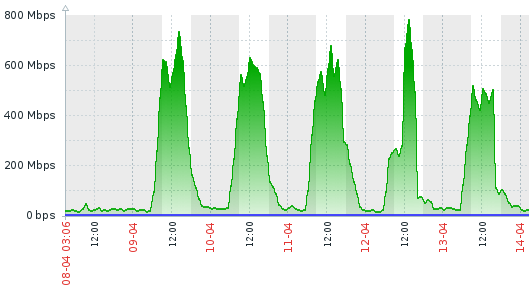
\includegraphics[scale=.7]{trafego-rede.png}
\label{fig:trafego-rede}
\legend{Fonte: \cite{zabbix}}
\end{figure}

\subsection{Infraestrutura Definida para Testes} \label{sec:infraestrutura}
%Descrever o que foi utilizado:
%Ex: Equipamentos - Servidores, ....
%    Configuração
%    Ferramentas - Snort (referenciar capítulo), ...

No ambiente de teste foi usado uma máquina Dell com 134 Megabytes (MB) de memória RAM e 40 núcleos. Usou-se XenServer \cite{xenserver} versão 7, sistema operacional (SO) \textit{opensource} da Citrix voltado para virtualização. Foram testados outros SOs porém somente o XenServer possuía, na época da instalação do ambiente, \textit{firmware} da placa de rede do \textit{host} compatível e que funcionava com instabilidade. 
 
Outro fator que pesou na escolha do SO foi a experiência com a plataforma e por existir uma interface para gerencia chamada XenCenter que roda no Windows. Uma alternativa \textit{opensource} desse software é o OpenXenManager que funciona nos sistemas Unix \cite{openxenmanager}.

No primeiro momento, foi instalado uma máquina virtual com o sistema operacional Debian 9.3 \textit{codename} Stretch \cite{debianwheezy}, uma distribuição linux com uma proposta de ser totalmente livre, usada como base para instalação de outras máquinas utilizando o recurso de \textit{snapshot}, uma cópia de uma máquina virtual rodando em um certo momento, do XenServer. O uso desse recurso foi necessário para criar um ambiente igual para as ferramentas em estudo.

Foi alocado 8 MB memória RAM, 4 processadores e 100 Gigabytes(GB) de espaço em disco para o \textit{snapshot}. Esses valores foram definidos com base em um estudo \cite{mikelococo} que considera vários fatores, como largura da rede, localização do IDS e versão, tipo do capturador de tráfego e tamanho da base de assinaturas para dimensionar os recursos de memória e processamento, aplicado especificamente ao Snort. A mesma regra foi aplicada ao Suricata.

Para o \textit{host} conseguir pegar o pacotes destinados a rede escolhida para o experimento, foi necessário uma configuração de espelhamento no roteador B (Figura \ref{fig:infra-ambiente}) que consiste na copia dos pacotes que saem pela porta dessa rede no roteador para a porta conectada no \textit{host} que possui uma largura de banda de 10 Gigabits. A interface de rede do \textit{host} precisou ser configurada no modo \textit{promisc}.

Posteriormente criou-se três máquinas virtuais, duas usadas para instalação dos IDSs (Suricata e Snort) e a terceira será usada para rodar o \textit{framework} Pytbull (\autoref{sec:pytbull}). Numa quarta máquina, instalou-se o sistema Kali Linux \cite{kalilinux} para geração de ataques, esse SO possui ferramentas nativas para testes de penetração e auditoria de segurança (Metasploit \autoref{sec:metasploit}, NMAP \autoref{sec:nmap} e OpenVAS \autoref{sec:openvas}). A infraestrutura final do ambiente de teste poder ser visualizada na \autoref{fig:infra-ambiente}.

\begin{figure}[!htb]
\centering
\caption{Infraestrutura do ambiente de teste}
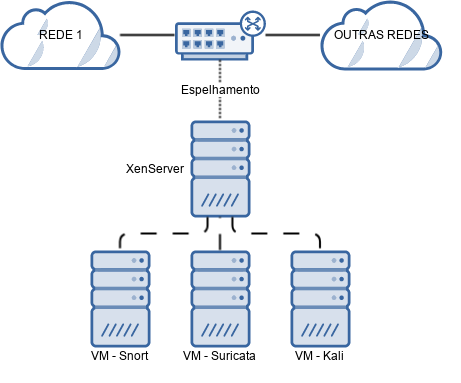
\includegraphics[scale=.65]{infra.png}
\label{fig:infra-ambiente}
\legend{Fonte: Autoria própria}
\end{figure}

Para coleta das informações de uso de recurso de hardware como memória, processamento e I/O das máquinas com os IDSs utilizou-se o \textit{daemon} Collectd \cite{collectd}. Outra opção para essa finalidade é a utilização de um servidor de monitoramento como o Zabbix \cite{zabbix}. A ideia de ter duas ferramentas para essa analise é fazer um comparativo e validar as informações coletadas.

O formato usado para facilitar a análise do \textit{logs} foi JavaScript Object Notation (JSON), um formato simples, leve e de fácil leitura. O Motor de Saída do Suricata já tem suporte a esse tipo de formato o que não acontece no Snort. Para tal, usou-se o IDSTools \cite{py-idstools}, uma coleção de bibliotecas na linguagem python que trabalha para auxiliar o IDS Snort. Dentre os utilitários presentes nessa coleção, temos o idstools-u2json, que converte, de forma continua, arquivo no formato unified2, uma das saídas disponível no Snort, para o formato JSON.

Para analisar os \textit{logs}, usou-se uma infraestrutura que combina três ferramentas:

\begin{alineas}
\item \textbf{Kibana} \cite{kibana}: Uma plataforma de análise e visualização desenhada para trabalhar com os índices do Elasticsearch \cite{elasticsearch}, a grosso modo, podemos dizer que ela é uma interface gráfica para o Elasticsearch. 
\item \textbf{Elasticsearch}: Um motor de busca e análise altamente escalável, capaz de armazenar, buscar e analisar uma grande quantidade de dados em tempo próximo ao real. 
\item \textbf{Logstach} \cite{logstach}: Um motor de coleta de dados em tempo real, unificando os dados de diferentes fontes dinamicamente, normalizando-os nos destinos escolhidos.
\end{alineas}

Dessa forma centralizou-se os \textit{logs}, facilitando a visualização e analise das ocorrências geradas pelos IDSs. 

\section{Testes Realizados} \label{sec:testes}
%Quais os testes realizados com justificativa ?
%Descrição dos testes. Quais os testes foram realizados ?
Os testes realizados são simulações de passos que uma pessoa má-intencionada iria tomar para alguma tentativa de invasão, entende-se por invasão, qualquer tipo de violação e alteração não autorizada de um serviço ou \textit{host}.

O passo inicial seria um estudo do alvo utilizando várias técnicas mas principalmente a engenharia social, analisando as pessoas que trabalharam na organização, enviando spam e \textit{phishing} na tentativa de capturar dados como senhas de acesso. 

Posteriormente, o atacante iria observar o tráfego da rede, verificando os serviços que o alvo oferece, a procura de alguma senha desprotegida (não criptografada). Esse passo inicial não será aplicados nos testes pois seria impossível o IDS detectar.

O passo seguinte seria uma garimpagem de informações e mapeamento da rede, a procura de um \textit{host} vulnerável. A ferramenta escolhida para essa finalidade é o Nmap (\autoref{sec:nmap}). 

No primeiro teste de \textit{scan}, usou-se o parâmetro '-F', habilitando a modo \textit{fast} do Nmap. Nesse modo, são verificadas apenas as portas especificadas no arquivo nmap-services, que, na instalação padrão, possui 27372 portas descritas. Isso é muito mais rápido que verificar todas as 65535 portas tcp e 65535 portas udp, possíveis em um \textit{host}. Abaixo segue o comando usado.

\begin{lstlisting}[caption={Comando NMAP no modo \textit{fast}},language=bash, frame=single, label={lst:nmap-F}]
    nmap -F 200.239.72.19
\end{lstlisting}

O segundo teste, usou-se o parâmetro '-A' do NMAP. Essa opção habilita opções adicionais avançadas e agressivas, descobrindo versões dos serviço, determinando protocolos de serviços, o nome da aplicação, o número da versão, o nome do \textit{host} (utilizando o DNS reverso), tipo de dispositivo, sistema operacional, entre outras informações. Ter um número de versão exacto ajuda substancialmente na determinação de quais \textit{exploits} o servidor está vulnerável \cite{nmap}.

\begin{lstlisting}[caption={Comando NMAP no modo de descoberta de versões},language=bash, frame=single, label={lst:nmap-sv}]  
    nmap -A 200.239.72.19
\end{lstlisting}

Uma forma encontrada para automatizar o processo de execução dos comandos citados acima foi a criação de um código em \textit{shell script}. O \textit{Shell Script} é uma linguagem de script usada por vários sistemas operacional, principalmente os baseados em UNIX. Abaixo segue o código.

\begin{lstlisting}[caption={Automatização das execuções do comando NMAP},language=bash, frame=single, label={lst:script-nmap}]
#!/bin/bash

echo "\nIniciando ..."
STARTIME=$(date)

for i in $(seq 1 100)
    do  
        echo "\n$i Execução..."
        nmap $1 200.239.72.19 > /dev/null
        sleep 5
    done

ENDTIME=$(date)                                                                                                                                                                 
echo "\nInicio $STARTIME"
echo "\nFim $ENDTIME"
\end{lstlisting}

Na primeira linha de um código em \textit{shell script}, precisamos especificar o interpretador utilizado (\#!/bin/bash). Criou-se duas variáveis, uma para armazenar a hora do inicio do \textit{script} e uma para armazenar termino, dessa forma, a pesquisa pelos alertas gerados pelas ferramentas será menos dispendiosa. O comando NMAP foi colocado dentro de um laço \textit{for}, executado 100 vezes. 

De posse de um alvo em potencial, próximo passo seria rodar um \textit{scanner} de vulnerabilidade, em busca de brejas já conhecidas, e que, geralmente por descuido do administrador, não foi fechada. Essas brejas podem ter várias origens, desde uma versão do serviço com \textit{bugs} ou uma má configuração. Para esse teste, usou-se o OpenVAS (\autoref{sec:openvas}).

É necessário algumas configurações no \textit{scanner} nessa etapa. Primeiramente, deve-se definir o alvo, tal configuração é feita através do caminho "\textit{Configuration > New target}", a \autoref{fig:openvas-newtarget} mostra a janela aberta, nela temos que definir um nome para o alvo e o IP ou a faixa de IP's, as outras configurações serão deixadas com o padrão.

\begin{figure}[!htb]
\centering
\caption{Definição do alvo no OpenVAS}
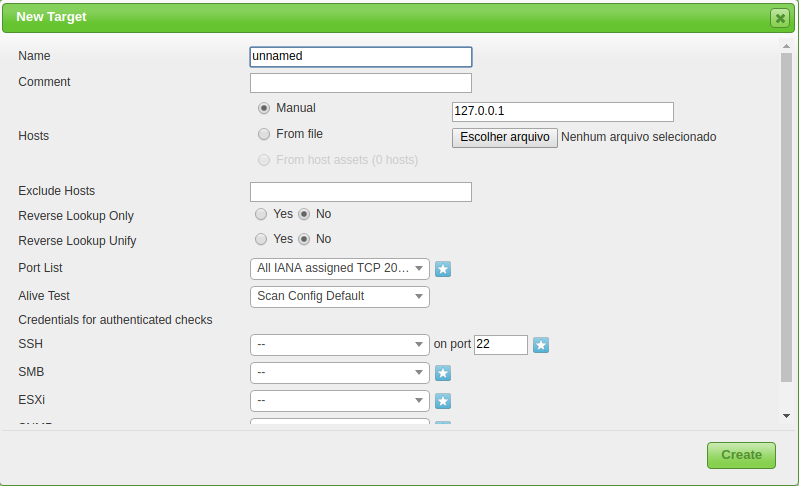
\includegraphics[scale=.55]{openvas-newtarget.png}
\label{fig:openvas-newtarget}
\legend{Fonte: Autoria própria}
\end{figure}

A realização do scan é feita através do caminho "\textit{Scans > Tasks > New Task}", na \autoref{fig:openvas-newtask} mostra a janela aberta, nela precisamos definir no nome da \textit{task} e o alvo, que foi definido anteriormente, as outras opções serão deixadas com o padrão. 

Por padrão, quando uma \textit{task} é criada, o \textit{scan} é automaticamente executado. Esse processo pode demorar, isso depende de quantos alvos foram definidos. Ao final, um relatório é exibido com as vulnerabilidades encontradas e categorizadas (\textit{high, medium, low}) de acordo com a sua severidade. Além disso, o OpenVAS exibe um sumário, descrevendo a(s) falha(s) encontrada(s) e como resolver ou mitigar o problema.

\begin{figure}[!htb]
\centering
\caption{Configuração de um \textit{task} de scan no OpenVAS}
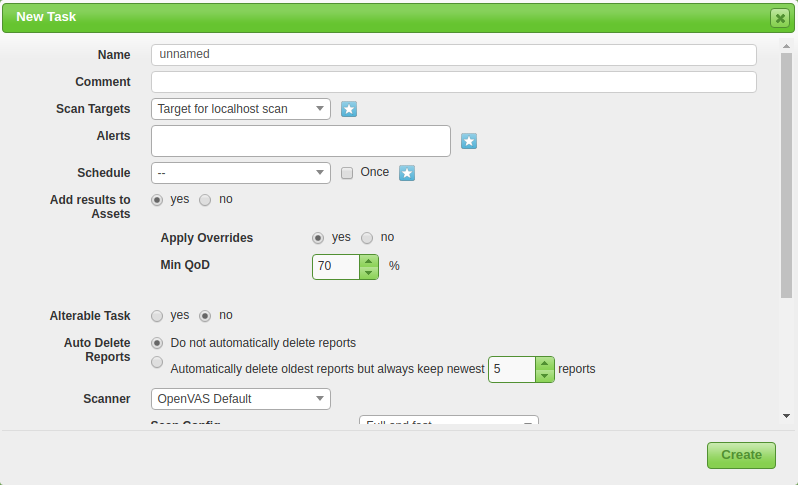
\includegraphics[scale=.55]{openvas-newtask.png}
\label{fig:openvas-newtask}
\legend{Fonte: Autoria própria}
\end{figure}

Outro teste realizado determinará a capacidade das ferramentas de detectar ataques de negação de serviço (\autoref{sec:negação}). Existem várias técnicas para realizar esse tipo de ataque, o usado nesse trabalho foi o TCP SYN FLOOD. 

Quando um cliente tenta começar um conexão TCP com um servidor, são trocados, entre eles, uma série de mensagens (\textit{Three-Way Handshaker}). O TCP SYN FLOOD consiste em enviar uma sequência de requisições SYN para o alvo, sobrecarregando-o diretamente na camada de transporte e indiretamente na camada de aplicação.

Para tal, usou-se o Metasploit Framework (\autoref{sec:metasploit}). Primeiramente, entrou-se no console de linha de comando, para acessar, basta, no terminal, digitar \textit{msfconsole}. Existe um modulo no Metasploit chamado \textit{synflood}, para utilizar esse modulo, é necessário definir o IP do alvo e o IP de onde partirá o ataque. Abaixo segue os comandos usados no \textit{msfconsole}.

\begin{lstlisting}[caption={Comando usados no Metasploit para ataque de negação de serviço},language=bash, frame=single, label={lst:synflood}]
use auxiliary/dos/tcp/synflood

msf auxiliary(synflood) > set rhost 200.239.72.19 (target IP)

msf auxiliary(synflood) > set shost 10.15.10.20 (attack IP)

msf auxiliary(synflood) > exploit
\end{lstlisting}

No ultimo teste, utilizou-se o \textit{framework} Pytbull (\autoref{sec:pytbull}). O Pytbull foi desenvolvido especificamente para realizar testes e validar configurações em IDPS. A documentação oficial exemplifica algumas arquiteturas que podem ser usadas, nesse trabalho usou-se a arquitetura \textit{remote mode} onde o IDS é colocado para escutar todo o tráfego que passa no \textit{switch} através de uma porta espelhada e com uma interface configurada em modo \textit{promisc}.

Por padrão, todos os testes do \textit{framework} estão ativados. Como o teste de DoS foi realizado utilizando o Metasploit, e para diminuir o tempo da experimentação, o módulo denialOfService do Pytbull foi desativado. Outro módulo desativado, devido demora na execução, foi o testRules, a execução desse módulo levava mais de uma hora. Para desativar esses módulos precisa-se editar o arquivo \textbf{pytbull/config/config.cfg}, alterando, na parte dos testes, os valores de 1 para 0.

Outra mudança feita, somente nessa fase, com o intuito de melhorar a eficácia do teste, foi a configuração das ferramentas de IDPS para analisar somente pacotes com o IP do \textit{host} que executará o Pytbull. 

Antes de executar o \textit{framework}, é necessário mover, para os \textit{hosts} que estão executando as ferramentas de IDPS, o script \textbf{pytbull/server/pytbull-server.py} encontrado no arquivo .tar.bz2, baixado no site oficial do Pytbull \cite{pytbull}. Esse executável abre um shell reverso no servidor que é usado pelo módulo clientSideAttacks do Pytbull, fazendo-o baixar arquivos maliciosos da Internet. 

Feito isso, basta executar os comandos abaixo, substituindo \textbf{suricata} e \textbf{snort} pelos seus respectivos IPs:

\begin{lstlisting}[caption={Comandos usados para execução do Pytbull}, language=bash, frame=single, label={lst:pytbull}]
cd pytbull/

sudo ./pytbull -t suricata

sudo ./pytbull -t snort
\end{lstlisting}

\section{Resultados} \label{sec:resultados}
%Resultados esperados e obtidos
%Quais os resultados dos testes ??
%Comparação das ferramentas
%Problemas encontrados
O Snort e Suricata são Sistemas de Detecção de Intrusão baseados em assinaturas, ambos gratuitos e multiplataformas, no entanto, caso queira uma base de assinaturas robusta e com suporte, o mesmo deve ser adquirido mediante a um pagamento. 

Nada impede o desenvolvimento de uma base própria, no entanto, é necessário uma equipe altamente capacitada e dedicada para esse fim, visto que, diariamente, são lançados na rede novos ataques ou variações de ataques existentes, tornando a atualização da base de assinaturas um processo árduo e custoso.

O Snort encontra-se consolidado no mercado há vários anos e com muitas versões, já o Suricata surgiu em 2010 como um novo motor, com a tecnologia \texit{multithreading} (processa várias tarefas ao mesmo tempo), aproveitando o paradigma multinúcleos dos processadores. Por esse motivo, espera-se que o desempenho do Suricata seja superior ao do Snort.

Foram encontrados vários desafios durante o desenvolvimento desse trabalho. Dentre elas, destacam-se a dificuldade de encontrar material e experimentos referente ao Suricata, a documentação oficial do sistema é pobre de conteúdo, limitando-se ao básico de instalação e algumas particularidades de configuração. 

Outra dificuldade que se destaca foi com relação a configuração do cenário de teste, devido a alta complexidade e por requerer configurações em vários equipamento, no qual, em alguns casos, a gerência pertencia a terceiros. Depois de um tempo, observou-se que nem todos os pacotes da interface espelhada estava passando para as VM's, isso afetaria os resultados dos testes. Após análise, concluiu-se que era necessário uma configuração de espelhamento no \textit{openvswitch} (utilizado pelo XenServer) do \textit{host}. 

As métricas usadas para análise e comparação das ferramentas são a utilização dos recursos de \textit{hardware} (memória, processamento), taxa de detecção, independente de ser falso positivo e falso negativo. No primeiro momento, havia a ideia de comparar utilizando essa métrica, no entanto, devido a uma quantidade muito grande de alertas e devido a rede ser grande (vários clientes), essa comparação tornou-se inviável.

No primeiro experimento realizado, utilizando o NMAP no modo \textit{fast}, a execução do \textit{script} \autoref{lst:script-nmap}, gerou um total de 62 alertas, dos quais 100\% deles foram do Snort. o Snort teve um desempenho melhor pois ele foi capaz de detectar a execução do comando.

No segundo teste de varredura, utilizando o NMAP no modo no qual é possível identificar as versões dos serviços e até o SO do alvo, as ferramentas geraram, com a execução do \textit{script} (\autoref{lst:script-nmap}), um total de 210 alertas, desses, 106 (50.5\%) foi gerado pelo Suricata e 104 (49.5\%) pelo Snort. Nesse cenário, houve quase uma equidade na taxa de detecção. No geral, nesse experimento com NMAP, o Snort teve um desempenho melhor, pois conseguiu gerar alertas no primeiro teste.

Já no teste realizado usando um \textit{scan} de vulnerabilidade (\autoref{sec:openvas}), os IDPS's geraram um total de 3071 alertas, sendo que 2142 (69.74\%) veio do Suricata e 929 (30.26\%) do Snort. Aqui, houve uma disparidade grande na taxa de detecção, assim, nesse cenário, o Suricata apresentou um desempenho melhor.

Para determinar se os IDPS's tinham capacidade de identificar ataques de negação de serviço utilizou-se um módulo do \textit{Metasploit Framework} (\autoref{lst:synflood}). Nesse teste, nenhuma uma das ferramentas alertou sobre a execução desse tipo de ataque. 

Por último, temos o teste utilizando \textit{framework} Pytbull (\autoref{lst:pytbull}). Para melhorar os resultados, configurou-se os IDPS's para apenas gerar alertas de eventos relacionados ao \textit{host} alvo. O resultado mostrou que houve um igualdade na taxa de detecção total, no entanto, o Suricata mostrou-se superior pois a quantidade não detectado do Snort foi maior, 81\% contra 47\% do Suricata. Abaixo segue os resultados, o gráfico é fornecido pelo próprio Pytbull ao final da execução. 

\begin{figure}[!htb]
\centering
\caption{Resultado da execução do \textit{framework} Pytbull sobre o Suricata}
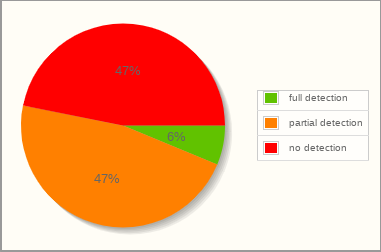
\includegraphics[scale=.7]{suricata-pytbull-report.png}
\label{fig:suricata-pytbull-report}
\legend{Fonte: Pytbull}
\end{figure}

\begin{figure}[!htb]
\centering
\caption{Resultado da execução do \textit{framework} Pytbull sobre o Snort}
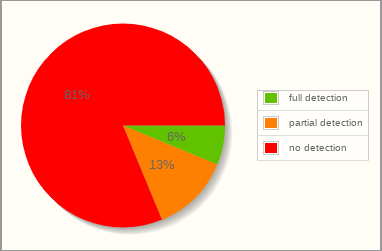
\includegraphics[scale=.7]{snort-pytbull-report.png}
\label{fig:snort-pytbull-report}
\legend{Fonte: Pytbull}
\end{figure}

Na \autoref{tab:suricata-recursos} está presente os dados coletados pelo serviço de monitoramento Zabbix do Suricata no decorrer de um mês. Foram coletados quatro informações, a carga do processador por núcleo nos tempos de um, cinco e quinze minutos e o uso de memória. Na \autoref{tab:snort-recursos}, há as mesmas informações, no entanto, do Snort.

Quanto a utilização de recurso de \textit{hardware}, conclui-se que o Snort utiliza um quantidade menor de memória, no entanto, possui um média de carga de processamento maior. Tal característica é válida devido a arquitetura do Snort usar apenas uma \textit{thread} por processo. O fato do processamento minimo do Suricata ser zero, dar-se a um comportamento da ferramenta, no qual o mesmo era finalizado de forma inesperada.  

\begin{table}[!htb]
\ABNTEXfontereduzida
\centering
\caption{Resultado do uso de recurso de \textit{hardware} do Suricata}
\label{tab:suricata-recursos}
\begin{tabular}{|M{5cm}|M{2cm}|M{2cm}|M{2cm}|}
    \hline
     & \textbf{minimo} & \textbf{média} & \textbf{máximo} \\
    \hline
    Carga do Processador (1 min) por core & 0 & 0.0326 & 0.545 \\
    \hline
    Carga do Processador (5 min) por core & 0 & 0.0326 & 0.545 \\
    \hline
    Carga do Processador (15 min) por core & 0 & 0.0326 & 0.545 \\
    \hline
    Uso de Memória & 3.16 GB & 5.48 GB & 7.78 GB \\
    \hline
\end{tabular}
\legend{Fonte: Zabbix} 
\end{table}

\begin{table}[!htb]
\ABNTEXfontereduzida
\centering
\caption{Resultado do uso de recurso de \textit{hardware} do Snort}
\label{tab:snort-recursos}
\begin{tabular}{|M{5cm}|M{2cm}|M{2cm}|M{2cm}|}
    \hline
     & \textbf{minimo} & \textbf{média} & \textbf{máximo} \\
    \hline
    Carga do Processador (1 min) por core & 0 & 0.1798 & 0.4625 \\
    \hline
    Carga do Processador (5 min) por core & 0.0075 & 0.1788 & 0.3225 \\
    \hline
    Carga do Processador (15 min) por core & 0.0125 & 0.1774 & 0.2825 \\
    \hline
    Uso de Memória & 2.09 GB & 3.81 GB & 5.06 GB \\
    \hline
\end{tabular}
\legend{Fonte: Zabbix} 
\end{table}

Quanto a taxa de detecção, analisou-se os registros de alertas gerados no Kibana, selecionando um período de uma semana. Houve um total de 47.778 de alertas gerados, desses 30.097 (62.99\%) vieram do Suricata e 17.681 (37.01\%) do Snort. Assim, o Suricata teve um desempenho melhor neste cenário. Vale salientar que, não esta sendo levado em consideração se o alerta é um falso negativo ou falso positivo.

\section{Conclusão} \label{sec:conclusão}
%A ferramentas estudas apresentaram resultados semelhantes. 
%\section{Métricas de Comparação}
%Consumo dos Recursos de Hardware (Memória, Processamento)
%Taxa de Detecção
%Número de Falsos Positivos/Negativos

Esse capítulo apresentou o cenário no qual as ferramentas estudas foram colocadas para análise. Descreveu-se a infraestrutura montada e os componentes envolvidos para a realização do estudo. Além disso, foi detalhado os testes realizados, simulações de ataques a uma máquina alvo dentro da rede e ao final os resultados obtidos. 

\chapter{Considerações Finais e Trabalhos Futuros} \label{ch:considerações}

Foram encontrados vários desafios durante o desenvolvimento desse trabalho. Dentre elas, destacam-se a dificuldade de encontrar material e experimentos referente ao Suricata, a documentação oficial do sistema é pobre de conteúdo, limitando-se ao básico de instalação e algumas particularidades de configuração. 

Outra dificuldade que se destaca foi com relação a configuração do cenário de teste, devido a alta complexidade e por requerer configurações em vários equipamento, no qual, em alguns casos, a gerência pertencia a terceiros. Depois de um tempo, observou-se que nem todos os pacotes da interface espelhada estava passando para as VM's, isso afetaria os resultados dos testes. Após análise, concluiu-se que era necessário uma configuração de espelhamento no \textit{openvswitch} (utilizado pelo XenServer) do \textit{host}.

Diante dos resultados obtidos na \autoref{sec:resultados}, conclui-se que, apesar da ferramenta Suricata (versão 4.0.0) ter, em aspectos gerais, um desempenho melhor, justificando assim, que a arquitetura nela implementada (utilizando \textit{multithread}) ajuda na melhoria da detecção e geração de alertas. 

No entanto, recomenda-se a utilização do Snort (versão 2.9.8.3) em um ambiente de produção real. Tal afirmação, é sustentada devido a um comportamento do Suricata observado durante o desenvolvimento desse trabalho, que, por algum motivo não investigado, era finalizado. Dessa forma, os alertas não eram gerados, deixando a rede um pouco desprotegida.

Além disso, caso opte-se por implantar o Suricata em um ambiente de produção, será necessário um esforço maior, pois a equipe de segurança, deve está sempre monitorando se o processo da ferramenta está executando e gerando os alertas corretamente.

A realização desse trabalho foi de grande valor para aquisição de conhecimento na área de segurança de redes. Concluindo-se que, embora haja na rede um IDS, somente a implementação deste não é suficiente para se ter uma segurança total, e sim, que ele deva atuar em paralelo com outros sistemas de segurança, vindo assim a somar na dura batalha pela obtenção de segurança em redes. 

Como trabalhos futuros, podemos avaliar as ferramentas em um ambiente mais controlado para tentar identificar se os alertas gerados são realmente de ataques lançado à rede. Assim, determinando a quantidade de falso negativos e falsos positivos e a precisão das ferramentas na geração de alertas.

\phantompart
\postextual
\bibliography{bib/dissertacao}
\phantompart
\printindex
\end{document}
